% Options for packages loaded elsewhere
\PassOptionsToPackage{unicode}{hyperref}
\PassOptionsToPackage{hyphens}{url}
\PassOptionsToPackage{dvipsnames,svgnames,x11names}{xcolor}
%
\documentclass[
  super,
  preprint,
  3p]{elsarticle}

\usepackage{amsmath,amssymb}
\usepackage{setspace}
\usepackage{iftex}
\ifPDFTeX
  \usepackage[T1]{fontenc}
  \usepackage[utf8]{inputenc}
  \usepackage{textcomp} % provide euro and other symbols
\else % if luatex or xetex
  \usepackage{unicode-math}
  \defaultfontfeatures{Scale=MatchLowercase}
  \defaultfontfeatures[\rmfamily]{Ligatures=TeX,Scale=1}
\fi
\usepackage{lmodern}
\ifPDFTeX\else  
    % xetex/luatex font selection
    \setmainfont[]{Comic Sans MS}
\fi
% Use upquote if available, for straight quotes in verbatim environments
\IfFileExists{upquote.sty}{\usepackage{upquote}}{}
\IfFileExists{microtype.sty}{% use microtype if available
  \usepackage[]{microtype}
  \UseMicrotypeSet[protrusion]{basicmath} % disable protrusion for tt fonts
}{}
\makeatletter
\@ifundefined{KOMAClassName}{% if non-KOMA class
  \IfFileExists{parskip.sty}{%
    \usepackage{parskip}
  }{% else
    \setlength{\parindent}{0pt}
    \setlength{\parskip}{6pt plus 2pt minus 1pt}}
}{% if KOMA class
  \KOMAoptions{parskip=half}}
\makeatother
\usepackage{xcolor}
\setlength{\emergencystretch}{3em} % prevent overfull lines
\setcounter{secnumdepth}{5}
% Make \paragraph and \subparagraph free-standing
\makeatletter
\ifx\paragraph\undefined\else
  \let\oldparagraph\paragraph
  \renewcommand{\paragraph}{
    \@ifstar
      \xxxParagraphStar
      \xxxParagraphNoStar
  }
  \newcommand{\xxxParagraphStar}[1]{\oldparagraph*{#1}\mbox{}}
  \newcommand{\xxxParagraphNoStar}[1]{\oldparagraph{#1}\mbox{}}
\fi
\ifx\subparagraph\undefined\else
  \let\oldsubparagraph\subparagraph
  \renewcommand{\subparagraph}{
    \@ifstar
      \xxxSubParagraphStar
      \xxxSubParagraphNoStar
  }
  \newcommand{\xxxSubParagraphStar}[1]{\oldsubparagraph*{#1}\mbox{}}
  \newcommand{\xxxSubParagraphNoStar}[1]{\oldsubparagraph{#1}\mbox{}}
\fi
\makeatother


\providecommand{\tightlist}{%
  \setlength{\itemsep}{0pt}\setlength{\parskip}{0pt}}\usepackage{longtable,booktabs,array}
\usepackage{calc} % for calculating minipage widths
% Correct order of tables after \paragraph or \subparagraph
\usepackage{etoolbox}
\makeatletter
\patchcmd\longtable{\par}{\if@noskipsec\mbox{}\fi\par}{}{}
\makeatother
% Allow footnotes in longtable head/foot
\IfFileExists{footnotehyper.sty}{\usepackage{footnotehyper}}{\usepackage{footnote}}
\makesavenoteenv{longtable}
\usepackage{graphicx}
\makeatletter
\def\maxwidth{\ifdim\Gin@nat@width>\linewidth\linewidth\else\Gin@nat@width\fi}
\def\maxheight{\ifdim\Gin@nat@height>\textheight\textheight\else\Gin@nat@height\fi}
\makeatother
% Scale images if necessary, so that they will not overflow the page
% margins by default, and it is still possible to overwrite the defaults
% using explicit options in \includegraphics[width, height, ...]{}
\setkeys{Gin}{width=\maxwidth,height=\maxheight,keepaspectratio}
% Set default figure placement to htbp
\makeatletter
\def\fps@figure{htbp}
\makeatother

\usepackage{lineno}
\usepackage{caption}
\makeatletter
\@ifpackageloaded{caption}{}{\usepackage{caption}}
\AtBeginDocument{%
\ifdefined\contentsname
  \renewcommand*\contentsname{Table of contents}
\else
  \newcommand\contentsname{Table of contents}
\fi
\ifdefined\listfigurename
  \renewcommand*\listfigurename{List of Figures}
\else
  \newcommand\listfigurename{List of Figures}
\fi
\ifdefined\listtablename
  \renewcommand*\listtablename{List of Tables}
\else
  \newcommand\listtablename{List of Tables}
\fi
\ifdefined\figurename
  \renewcommand*\figurename{Figure}
\else
  \newcommand\figurename{Figure}
\fi
\ifdefined\tablename
  \renewcommand*\tablename{Table}
\else
  \newcommand\tablename{Table}
\fi
}
\@ifpackageloaded{float}{}{\usepackage{float}}
\floatstyle{ruled}
\@ifundefined{c@chapter}{\newfloat{codelisting}{h}{lop}}{\newfloat{codelisting}{h}{lop}[chapter]}
\floatname{codelisting}{Listing}
\newcommand*\listoflistings{\listof{codelisting}{List of Listings}}
\makeatother
\makeatletter
\makeatother
\makeatletter
\@ifpackageloaded{caption}{}{\usepackage{caption}}
\@ifpackageloaded{subcaption}{}{\usepackage{subcaption}}
\makeatother
\journal{Elsevier}

\ifLuaTeX
  \usepackage{selnolig}  % disable illegal ligatures
\fi
\usepackage[]{natbib}
\bibliographystyle{elsarticle-num}
\usepackage{bookmark}

\IfFileExists{xurl.sty}{\usepackage{xurl}}{} % add URL line breaks if available
\urlstyle{same} % disable monospaced font for URLs
\hypersetup{
  pdftitle={Can graph similarity metrics be helpful for analogue identification as part of a read-across approach?},
  pdfauthor={Brett Hagan; Imran Shah; Grace Patlewicz},
  pdfkeywords={Read-Across, Graph similarity, Graph kernels, Graph
convolutional networks (GCNs)},
  colorlinks=true,
  linkcolor={blue},
  filecolor={Maroon},
  citecolor={Blue},
  urlcolor={Blue},
  pdfcreator={LaTeX via pandoc}}


\setlength{\parindent}{6pt}
\begin{document}

\begin{frontmatter}
\title{Can graph similarity metrics be helpful for analogue
identification as part of a read-across approach?}
\author[1,2]{Brett Hagan%
%
}

\author[2]{Imran Shah%
%
}

\author[]{Grace Patlewicz%
\corref{cor1}%
}


\affiliation[1]{organization={ORAU, Oak Ridge Associated
Universities},city={Oak Ridge},postcode={TN, USA},postcodesep={}}
\affiliation[2]{organization={Center for Computational Toxicology and
Exposure (CCTE), Office of Research and Development, US Environment
Protection Agency},addressline={109 TW Alexander Dr},city={Research
Triangle Park},postcode={NC 27711 USA},postcodesep={}}

\cortext[cor1]{Corresponding author}



        
\begin{abstract}
Read-across is a technique used to fill data gaps for substances lacking
specific hazard data. The technique relies on identifying source
analogues with relevant data that are `similar' to the substance of
interest (the target). Typically, source analogues are identified on the
basis of structural similarity but the evaluation of their suitability
for read-across depends on other contexts of similarity including their
physical property information, chemical reactivity, bioactivity and
metabolism. Whilst quantifying structural similarity is well
established, often relying on chemical fingerprints and using a
similarity index such as Tanimoto to limit the number of analogues
returned, characterising other aspects of similarity objectively remains
a challenge. Many different aspects of a substance and its associated
properties lend themselves to being represented by graphs which offers
alternative means by which analogues could be potentially identified and
evaluated for read-across purposes. This manuscript considered at least
three such methods; graph kernel, graph embedding, and deep learning
(DL) approaches and explored their utility for analogue identification
using 5 datasets of varying size and diversity. Comparisons were made
using two chemical fingerprint approaches, ToxPrints and Morgan
fingerprints.
\end{abstract}





\begin{keyword}
    Read-Across \sep Graph similarity \sep Graph kernels \sep 
    Graph convolutional networks (GCNs)
\end{keyword}
\end{frontmatter}
    

\setstretch{1.5}
\section{Introduction}\label{introduction}

\subsection{Background to Read-Across}\label{sec-background}

There are tens of thousands of substances that exist in active commerce
e.g.~the US Toxic Substances Control Act (TSCA) comprises
\textasciitilde42,000 substances, of which only a small proportion have
undergone sufficient toxicological evaluation. In a recent EPA report
\citep{etap_2024}, only 15\% of substances in US commerce had been
subjected to any of the standard toxicity tests used to characterise
human health that assessing each chemical would present a significant
and impractical challenge in terms of cost, animal welfare, and
resources \citep{nrc_toxicity_1984}. \emph{In vitro} and \emph{in
silico} approaches have the potential to play a large role in
prioritising which chemicals to focus on in the absence of conventional
toxicity data. \emph{In silico} approaches encompass (quantitative)
structure-activity relationships ((Q)SAR) as well as read-across, both
of which relate chemical structure to (eco)toxicological or physical
property endpoints. QSARs are often used to address gaps for
environmental fate, ecotoxicological and physical property endpoints
whereas read-across is most commonly used for human health related
endpoints. To illustrate its significance for regulatory purposes,
read-across is cited as the most commonly used adaptation to address
information requirements under the European Union's Registration
Evaluation and Authorisation of Chemicals (REACH) regulation
\citep{eu_regulation_2006, macmillan_last_2024}.

In brief, read-across describes the method for filling a data gap
whereby a substance with existing data (termed the `source analogue') is
used to make a prediction of the same property for a `target' substance
with limited available empirical data. The approach relies on the
premise that both source and target substances are `similar' in some
context with relevant information pertaining to a specific outcome
\citep{enoch_chemical_2010, oecd_guidance_2014}. Key to this approach is
the characterisation of similarity. Although structural similarity is
the most common approach used to identify candidate source analogues,
other similarity contexts such as similarity in physicochemical
properties, metabolism, chemical reactivity, bioactivity and
toxicological profile also play a significant role in justifying the
relevance and suitability of those source analogues for read-across. For
example, metabolic similarity might entail an assessment of the
similarity of transformation pathways or the commonality of metabolites
formed as determined in experimental studies. Physicochemical similarity
might compare certain physical property information such as the log of
the octanol-water partition coefficient (logKow), melting point, boiling
point etc. of source analogues relative to the target substance to
determine whether physical form and partitioning are likely to be the
same. Similarity in toxicity might evaluate whether the available
empirical data identifies the same target organs impacted and whether
the potencies are comparable or follow a specific trend. Such similarity
context assessments are largely qualitative and heavily reliant on
expert judgement in concert with empirical data
\citep{patlewicz_building_2015}. This does result in challenges in terms
of reproducibility, scalability and acceptance for regulatory purposes
\citep{shah_systematically_2016}. Indeed, read-across as a technique has
been in use for \textasciitilde25 years, but acceptance for certain
regulatory contexts (e.g.~risk assessment) or within specific
jurisdictions still remains variable \citep{patlewicz_towards_2023}.
Thus, progress towards approaches that may increase confidence in and
reduce the levels of inherent uncertainty in read-across predictions
continue to be a focus of ongoing research.

Significant effort has been directed towards the evaluation of
confidence in analogue identification and evaluation across a wide range
of studies
\citep{patlewicz_building_2015, blackburn_framework_2014, schultz_assessing_2019, wu_framework_2010, patlewicz_navigating_2018}.
Several have aimed to define frameworks for characterising uncertainty
\citep{schultz_assessing_2019, schultz_strategy_2015, blackburn_framework_2014, patlewicz_navigating_2018},
whereas others have demonstrated how high-throughput screening data can
be helpful in substantiating mechanistic or biological similarity within
read-across justifications
\citep{escher_towards_2019, patlewicz_navigating_2018, rovida_nam-supported_2021}.
The European Chemicals Agency (ECHA) have developed a read-across
assessment framework in an effort to improve the characterisation and
documentation of read-across uncertainties
\citep{european_chemicals_agency_read-across_2017} whereas the
Organisation of Economic and Co-operative Development (OECD) have been
facilitating the development of case studies with the aim of updating
existing grouping technical guidance \citep{oecd_guidance_2014} with one
focus being on reducing read-across uncertainties \citep{OECD_IATA}. In
our own work, Generalised Read-Across (GenRA)
\citep{shah_systematically_2016, patlewicz_towards_2023} was created
with the goals of quantifying performance and uncertainty by
establishing performance baselines and quantifying the contribution that
different similarity contexts play in identifying source analogues and
making toxicity predictions. Research has continued to evaluate the
impact that different types of similarity play in read-across for the
prediction of \emph{in vivo} toxicity outcomes
\citep{patlewicz_systematic_2024, tate_repeat-dose_2021, helman_extending_2018, nelms_mechanistic_2018, boyce_comparing_2022}
together with implementing the insights gained in the GenRA
(www.comptox.gov/genra) web application
\citep{patlewicz_towards_2023, shah_genra_2024}.

\subsection{Source analogue
identification}\label{source-analogue-identification}

There are a number of software tools that facilitate the identification
of source analogues. Most of these use structural similarity as a basis
to return analogues. This is usually performed in one of two main ways -
either by a descriptor-based similarity calculation or a
substructure-based assessment \citep{kunimoto_maximum_2016}. In
practice, this means that a software tool contains a large database (or
dataset) of chemical substances that serves as a source analogue
inventory. To identify analogues, a search query is performed using the
target substance of interest to return candidate analogues. In a
substructure-based approach, a determination of the substructures shared
with the target substance are made or matched molecular pairs
\citep{oboyle_using_2014, noauthor_matched_2021} are generated to
identify common core structures that are distinguished at a given site.
Such substructure-based calculations are binary - either the target and
source analogues share a pre-defined substructure or not, therefore no
adjustable threshold exists to tune the returned set of candidate
analogues. On the other hand, the hits returned are often more
chemically intuitive and interpretable.

In a descriptor-based approach, the key considerations are how the
substances forming the source inventory are represented numerically and
what metric is used to quantify a specific threshold of similarity.
Source analogues can be characterised by 1D, 2D or 3D representations of
structures or hybrids of these. The EPA CompTox Chemicals Dashboard
\citep{williams_comptox_2017},
\href{https://pubchem.ncbi.nlm.nih.gov/}{PubChem}, as well as the many
functionalities within the OECD Toolbox (qsartoolbox.org)
\citep{schultz_oecd_2018} facilitate such analogue searches. Two
dimensional binary chemical fingerprints are frequently used for
practical efficiency especially when a source inventory contains large
numbers of substances e.g.~1 million substances. A target substance will
then be converted into the same chemical fingerprint representation and
a query based on pairwise similarities will return a number of
candidates either based on the similarity threshold set or the
user-defined number of candidates. The similarity threshold is a
quantitative measure between 0 and 1 that summarises the commonality in
structure based on the presence and absence of particular chemical
fingerprints. By far, the most common similarity index that is used in
the Tanimoto (Jaccard) index \citep{bajusz_why_2015} though there are a
number of other similarity indices that can also be used
\citep{bajusz_why_2015, floris_generalizable_2014}. The choice of
similarity index depends on the chemical representation used. A Tanimoto
index lends itself to binary fingerprints whereas other metrics (as
outlined in Gallegos-Saliner et al\citep{saliner_ecb}) may be more
suitable in cases where continuous descriptors represent the source
analogues.

There are several types of chemical fingerprints, one of the most
popular the extended connectivity fingerprint (ECFP) or Morgan
fingerprint \citep{rogers_extended-connectivity_2010}. The ECFP defines
molecular features by assigning identifiers to each of the atoms in the
molecule based on some combination of properties such as atomic number,
atomic mass etc. Then each atom collects its identifier and those of its
neighbouring atoms into an array and uses a hash function to reduce the
array into a single integer identifier. This captures the neighbourhood
of the atom. Once all atoms have generated their new identifiers, these
are updated and the process is performed several times over. After each
iteration, the identifier contains information about the immediate
neighbours and then the neighbours of those neighbours and so on until
each atom will contain information from all parts of the molecule.
Finally the identifiers are converted into a bit array depending on the
length of the fingerprint array that the user has defined. ECFP4 is
probably the most common ECFP fingerprint where the 4 denotes the
largest possible fragment having a width of 4 bonds.

Another type of fingerprint is the key or dictionary fingerprint where
there is a defined fixed set of substructural features representing
molecular characteristics. MACCS (Molecular Access System by Molecular
Design Limited) \citep{durant_reoptimization_2002} and ChemoType
ToxPrints \citep{yang_new_2015} are examples of these. The MACCS
fingerprint was one of the first developed, containing 166 structural
features. The original ToxPrints comprised a set of 729 generic
structural fragments organised by atom, bond, chain, ring types as well
as specific chemical groups. Atom pairs forms another type of
fingerprint where an algorithm of atom typing is performed such that
certain values for each atom of a molecule is computed
\citep{carhart_atom_1985}. An atom pair is defined in terms of the
atomic environments of, and the shortest path separations between, all
pairs of atoms in the topological representation of a chemical
structure.

In each case, the fingerprint is usually represented as a bit string or
binary vector to denote presence and absence of a structural feature
that can then be used as a query to search for source analogues. Some
fingerprints can also encode counts to capture the number of occurrences
of a structural feature rather than just its presence or absence.

Chemical fingerprints have proved useful for fast similarity comparisons
as well as inputs into development of QSARs for different activity
outcomes including toxicity endpoints. The fingerprints themselves
represent a simplified representation of a chemical that may be
insufficient to resolve differences in toxicity outcomes that is
important in read-across. For example, Morgan circular fingerprints are
typically poor at perceiving global features of a molecule (e.g.~size or
shape) and may fail to discriminate between subtle changes between 2
small molecules. One particular issue with using Morgan fingerprints is
that whilst they reflect which substructures are present in a molecule,
their interconnectedness (particularly over large distances) is lost.
More details on the different types of structural representations can be
found in a recent review \citep{Banerjee_2024}.

This study took inspiration from Mellor et al
\citep{mellor_molecular_2019}, to evaluate whether considering the
inherent representation of a chemical structure as a molecular graph,
with atoms as nodes and bonds as edges, might offer novel ways of
characterising structural information and in turn similarity for
read-across.

\subsection{Topological indices}\label{topological-indices}

Of course, it important to acknowledge that considering chemicals as
molecular graphs is not a novel concept. In fact, a wide variety of
chemical properties and processes have been modelled using information
derived from molecular graphs for many decades. Traditional topological
indices for chemical structures are algebraic invariants of hydrogen
depleted molecular graphs which represent the topology of a molecule.
There are hundreds of topological indices but the majority can be
broadly categorised into 5 main types namely: degree-based indices,
distance-based indices, count-based indices, eigenvalue-based indices
and information-theoretic indices \citep{Alameri_2021}.

Degree indices are based on the degree of the nodes in the graph.
Historically, the Zagreb Index which is based on the degrees of the
nodes focusing on the sum of squares or products of node degrees was the
first degree based structural descriptor though developed for a
different purpose as described by Gutman \citep{gutman_2013}. The first
true degree based topological index was put forward by Randic in 1975
\citep{randic_1975}. The so-named Randic Index is defined by the sum of
the inverse of the square roots of the degrees of adjacent nodes. It is
possibly one of the most widely applied topological indices in
chemistry. Randic noted good correlation between the index and a number
of physicochemical properties of alkanes such as surface area, boiling
point. More information on the Randic index can be found in the
following review by Li and Shi \citep{li_2008}.

The most common distance based index is the Wiener Index, which
represents the sum of the shortest-path distances between all pairs of
nodes in the graph. Wiener demonstrated a correlation between the index
and boiling points of alkanes \citep{wiener_1947}. Count based indices
include the Hosoya Index which counts the number of matching sets in the
graph. The Hosoya index was first introduced in 1971 \citep{Hosoya_1971}
demonstrating correlations between boiling points of alkanes. Eigenvalue
based indices include the Estrada index which is the sum of the
exponential of the eigenvalues of the adjacency matrix. Initially it was
used to quantity the degree of folding of long chain molecules such as
proteins. Gutman et al \citep{IvanGutman2011} provided an extensive
survey on the Estrada index and its applications. Finally,
information-theoretic indices use concepts from information theory to
quantify the distribution of certain properties within the graph. The
Shannon entropy, one such example, measures the diversity in the
distribution of node degrees. It quantifies the complexity or diversity
of a molecule based on the distribution of different atom types within
its structure, essentially measuring the ``uncertainty'' in predicting
which type of atom will be found at a given position within the
molecule; a higher Shannon entropy indicates a greater variety of atom
types and a more complex structure. Information entropy in chemistry has
been extensively reviewed in Sabirov and Shepelvich
\citep{sabirov_information_2021}.

Topological indices have been widely and successfully applied to the
quantitative correlation of many different molecular properties notably
boiling point, chemical reactivity as well as biological activity
\citep{roy_use_2017, ramakrishnan_topological_2013}. Although the
indices have been used in many QSAR studies, one of their main
shortcomings has been a perceived lack of interpretability
\citep{todeschini_chemical_1992}.

\subsection{Graph Similarity}\label{graph-similarity}

Topological indices provide a single, composite number that
characterises each molecule's structure. Whilst this approach is
advantageous for its simplicity and efficiency, it often compresses
complex structural information into one value, which can obscure finer
details about specific molecular substructures. To address this, a
broader range of graph similarity methods have been developed, allowing
for more granular analysis. Techniques such as graph edit distance,
graph isomorphism, and maximum common subgraph matching offer a way to
directly compare molecular structures, identifying subtle differences
and shared features that single-index values may overlook
\citep{ullmann_algorithm_1976, pelillo_replicator_1999, melnik_similarity_2002, jeh_simrank_2002, zager_graph_2008, koutra_algorithms_2011, chartrand_graph_1998}.

\subsubsection{Graph edit distances using Reduced
graphs}\label{graph-edit-distances-using-reduced-graphs}

Reduced graphs provide a summarised representation of a chemical
structure that are produced by collapsing connected atoms into single
nodes and forming edges between the nodes in accordance with bonds in
the original structure. Reduced graphs have been used in a variety of
applications in chemoinformatics ranging from the representation and
search of Markush structures to the identification of structure-activity
relationships (SARs). There are a number of different graph reduction
schemes though each has been devised to address a different purpose
\citep{gillet_similarity_2003, birchall_reduced_2011, birchall_training_2006}.
Graph reduction schemes have been developed for similarity searching
often with the objective of identifying substances with similarity in
activity. Various methods have also been developed to quantify the
similarity between reduced graphs from fingerprint approaches, graph
matching as well as an edit distance method. The edit distance approach
quantifies the degree of similarity of 2 reduced graphs based on the
number and type of operations needed to convert one graph to the other.
One benefit of the edit distance method is the ability to assign
different weights to different operations - useful when deriving
activity specific weights as evidenced in Birchall et al.
\citep{birchall_training_2006}. However, graph edit distance are
computationally expensive unless approximation algorithms are used
particularly for larger graphs. Garcia-Hernandez et al. \citep{RN25}
employed graph edit distances to reduced graph representations to
estimate the bioactivity of a chemical on the basis of the bioactivity
of similar compounds and found better performance than the array
representation-based approaches they compared against.

\subsubsection{Graph isomorphism}\label{graph-isomorphism}

Several foundational questions of chemical similarity analysis have
often been framed as graph comparison problems; chemical equivalence may
be modelled as a graph isomorphism task, i.e.~are two chemical graphs
identical (isomorphic)? Another question may be to determine whether
some chemical graph is included as part of another chemical. Searching
for a specific substructure (e.g.~a benzene ring) within another
chemical has been modeled as a subgraph isomorphism task. The
enumeration of possible chemical structures is closely related to graph
enumeration \citep{RN22}. Graph isomorphism is a test of structural
equivalence, wherein two graphs are isomorphic if a structure exists
that preserves a one-to-one correspondence between the two graphs sets
of nodes and edges.

\subsubsection{Maximum common subgraph}\label{maximum-common-subgraph}

A common need in cheminformatics to the ability to align pairs of
molecules together to make a determination of the degree of structural
overlap. This is useful when exploring SARs, predicting bioactivity of
substances or identifying chemical reaction sites. The degree of overlap
between a pair of chemicals can be achieved using maximum common
subgraph isomorphism algorithms
\citep{duesbury_maximum_2017, raymond_maximum_2002}. In cheminformatics,
maximum common subgraph isomorphism is usually referred to as
identifying the maximum common substructure (MCS). Given two structures,
the MCS is the largest substructure common to both. Maximum could be
interpreted to imply the maximum number of atoms, number of bonds,
number of cycles or even some physical property. There are also
variations in how atom and bond equivalency might be defined. However,
the most common MCS is where all atoms are the same if the element
numbers are the same and the bonds are of the same type. There are a
range of algorithms that can determine the MCS between pairs of
chemicals. Some algorithms and perhaps the most prevalent work on the
basis of identifying cliques or maximal cliques. A clique is a set of
nodes in a graph such that each node is connected to each and every
other node, with a maximal clique in a graph being one that is not
contained within another large clique. Examples include the
Bron-Kerbosch algorithm \citep{bron_algorithm_1973} which reports all of
the maximal cliques found. TOPSIM \citep{durand_efficient_1999} is
another algorithm designed to find the Maximum Common Edge Subgraph
(MCES) between two graphs. The Maximum Common Edge Subgraph is similar
to the Maximum Common Subgraph (MCS) problem but focuses on finding the
largest subgraph that has the maximum number of edges in common between
the two graphs. In this case, the algorithm converts labelled graph
representations of two molecules into a compatibility graph. Then a
modified maximal clique algorithm is used to find the maximal clique
which represents the largest common substructure (excluding common
isolated atoms) for the two molecules. A maximal common substructure is
obtained by combining the largest common substructure and the common
isolated atoms. The size of a maximal common substructure is then used
to define both a molecular similarity index and a topological distance
for two molecules. Other types of algorithms include subgraph
enumeration algorithms which involve enumerating all connected subgraphs
common to the two graphs that are being compared and then returning the
largest subgraph. Raymond and Willett \citep{raymond_maximum_2002}
reviewed the main solutions for pairwise MCS including multiple MCS
\citep{dalke_fmcs_2013}.

Whilst methods such as the maximum common subgraph (MCS) excel at
pinpointing shared structural features in pairwise comparisons, they can
become computationally intensive and less scalable when applied to large
chemical datasets. To address some of these limitations, more recent
graph similarity approaches, such as graph kernel methods, graph
embeddings, and deep learning-based techniques, have been developed.
Graph kernel methods directly calculate a similarity score between two
graphs based on their structural properties. Graph embedding methods
transform graphs into numerical representations (vectors) that can be
compared using standard distance metrics. These techniques are both
unsupervised in that the representations are not tuned or customised for
any specific outcome such as toxicity. Deep learning methods, a subset
of graph embedding, learn these numerical representations using neural
networks using labelled data such that the embeddings reflect some
insights about the toxicity endpoint of interest.

\subsubsection{Graph Kernels}\label{graph-kernels}

Graph kernels were first introduced as a way to compare complex
structures like graphs based on a concept from Haussler's work on
kernels for discrete structures \citep{kondor_diffusion_2002}. The term
``graph kernels'' soon emerged to describe methods specifically for
comparing graphs \citep{RN27, RN45, scholkopf_fast_2007}. The core idea
behind graph kernels is to break down a graph into smaller components,
called substructures. These substructures are then used to create
feature vectors, which characterise the graph. By comparing these
feature vectors, it is possible to measure how similar two graphs are.
The inner products of the feature vectors can be efficiently computed to
produce a similarity score between the graphs. The key to graph kernels
lies in how the graph is decomposed. One simple approach is to count how
many node labels are shared between graphs and computing the inner
products of these label counts to produce a similarity score
\citep{kriege_survey_2020}. Figure~\ref{fig-count} provides a conceptual
example of counting node labels.

\begin{figure}

\centering{

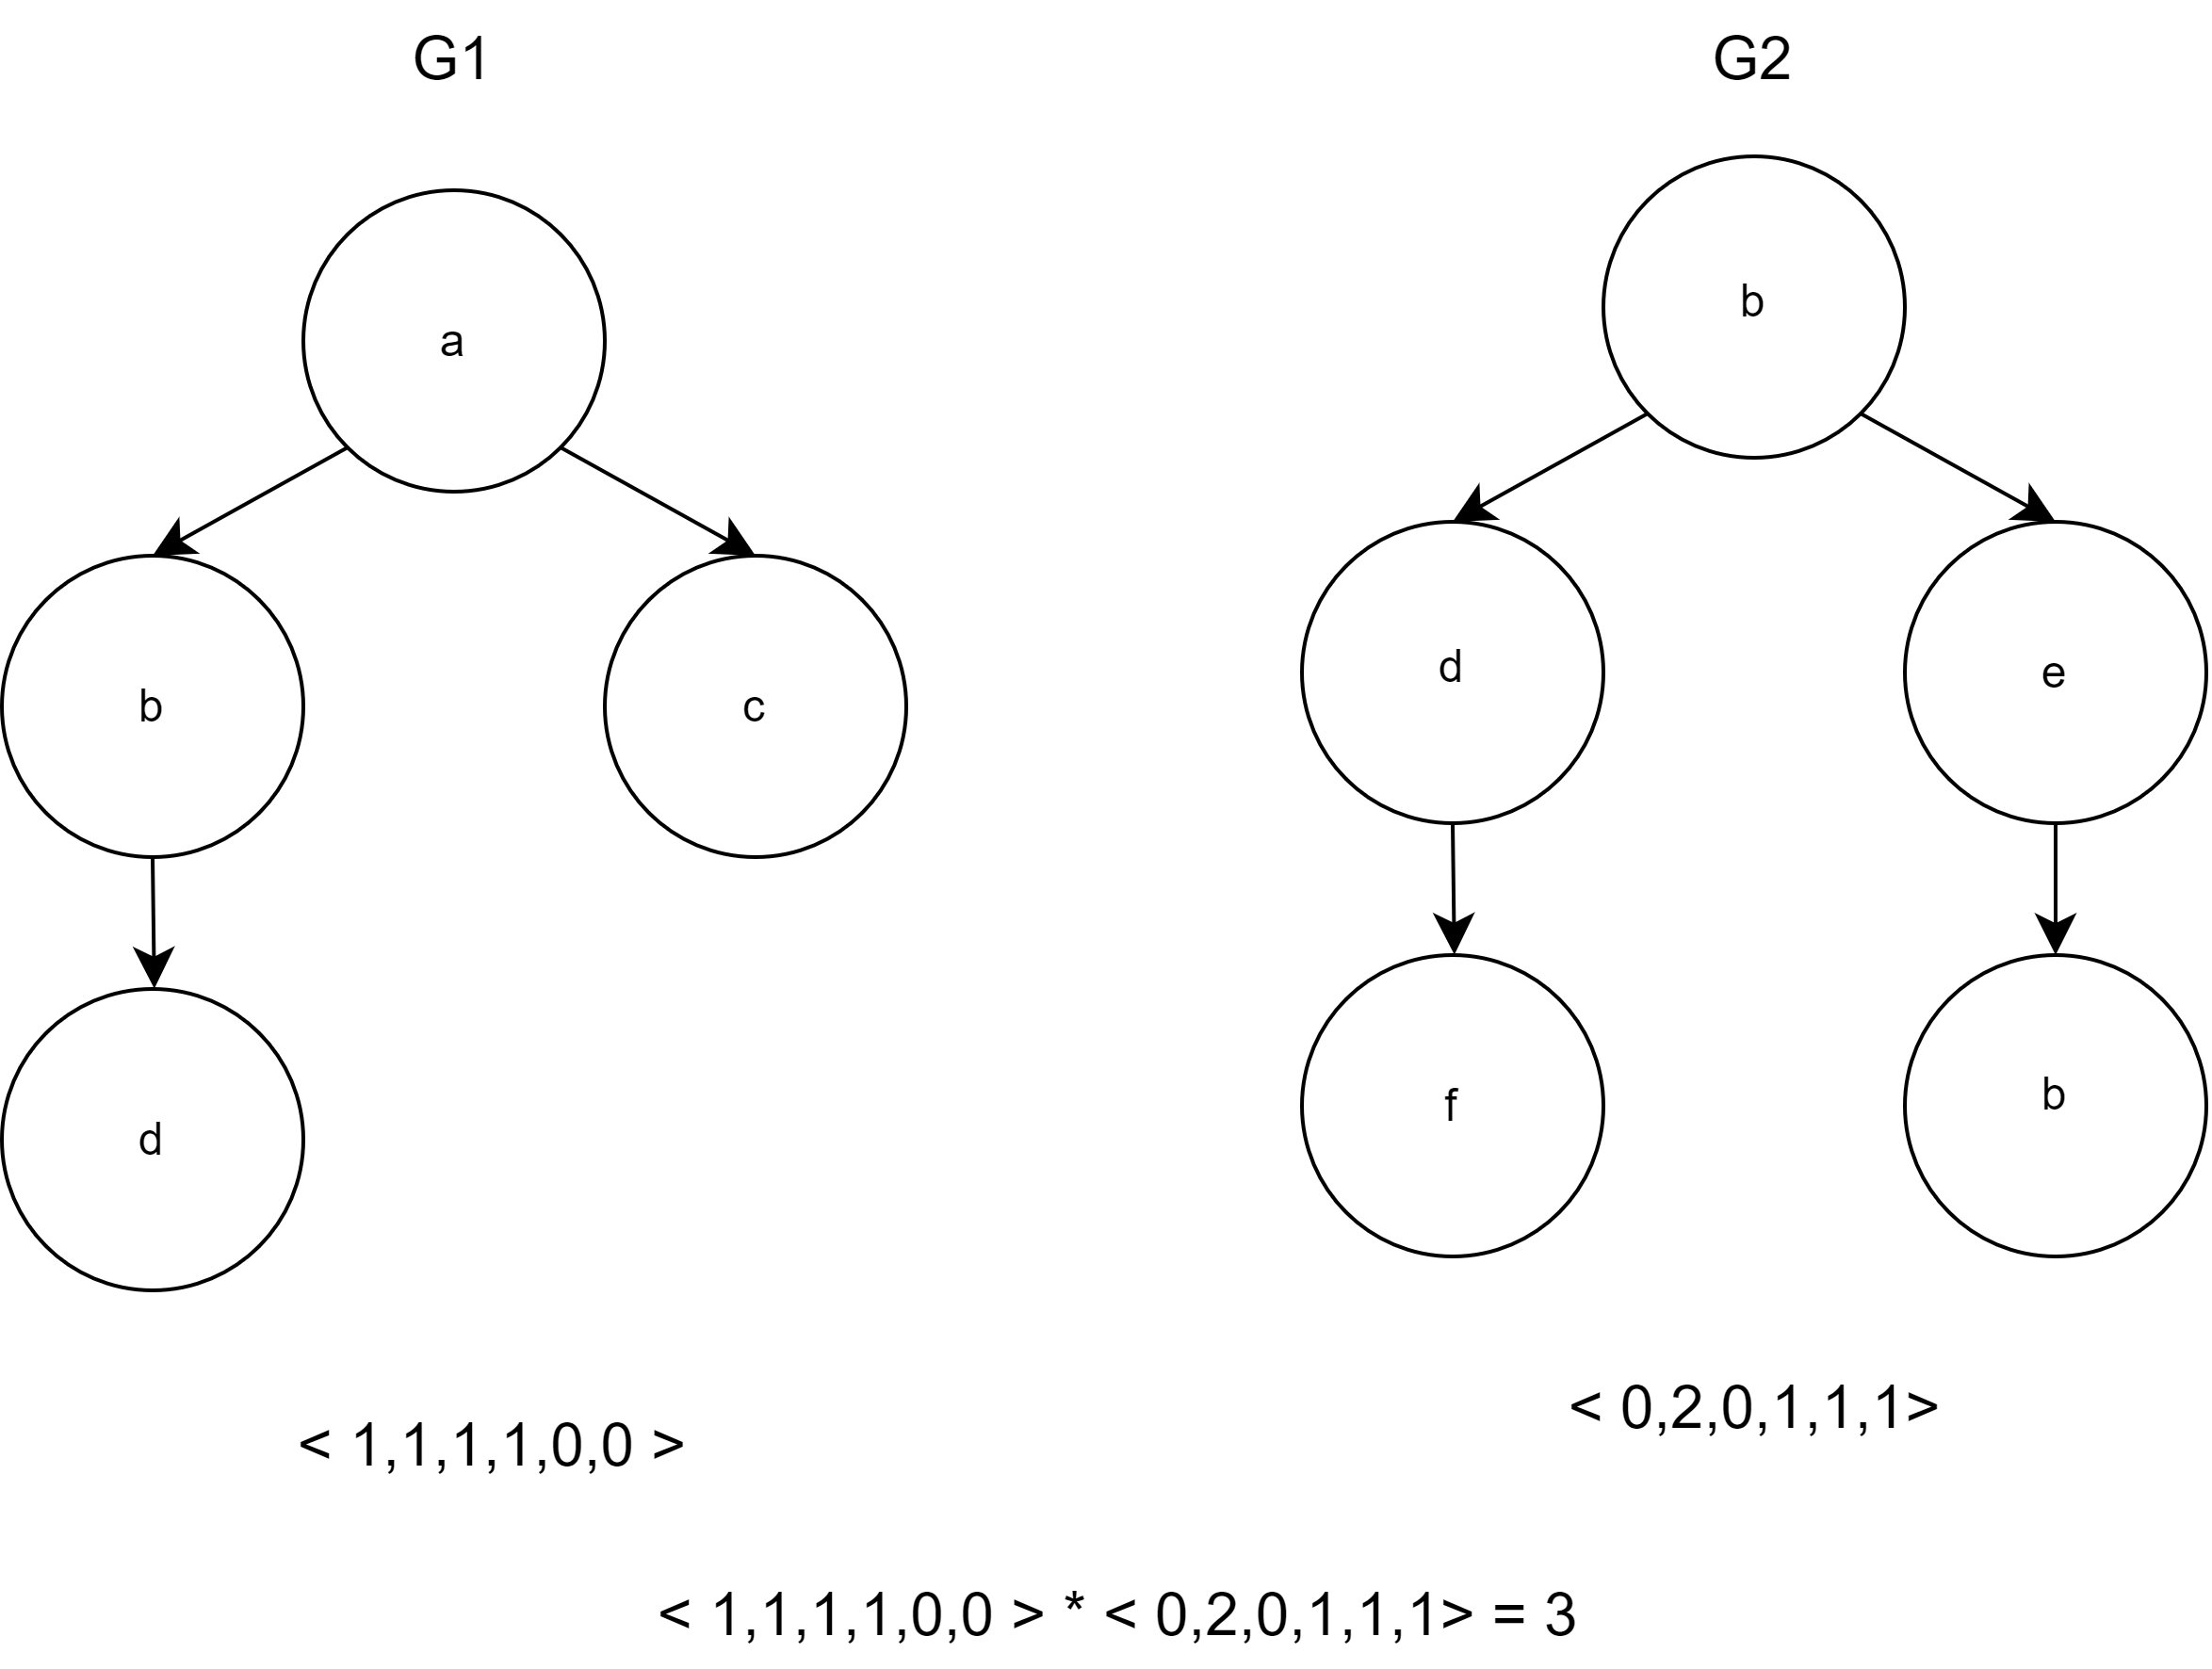
\includegraphics[width=1\textwidth,height=\textheight]{fig-count.png}

}

\caption{\label{fig-count}Graph kernel counting node labels. The feature
vectors for both graphs are constructed by counting the numbers of node
labels in each graph. A similarity score is then obtained by computing
the inner products of the feature vectors.}

\end{figure}%

There are many different ways to decompose a graph in order to compare
them. One approach is through random walk kernels. This method involves
taking random paths through the graph and counting how often each path
occurs in each graph \citep{gartner_survey_2003}. Shortest path kernels
aim to find the shortest paths between labelled nodes (atoms) in each
graph and using these to construct feature vectors \citep{RN30}. A more
advanced method builds on the Weisfeiler-Lehman (WL) graph isomorphism
heuristic that was introduced by Shervashidze in 2011; known as the WL
subtree kernel \citep{RN46}. The WL isomorphism heuristic works by
iteratively updating the labels of each atom based on the labels of its
neighbouring atoms. Over several iterations, this process captures more
detailed substructures within the molecule. This helps capture the
context of each atom in the molecule gradually embedding the molecular
structure into the labels. As the labels evolve, they encode
increasingly larger neighbourhoods around each atom. This means that the
WL kernel can capture structural features like functional groups that
are shared between molecules. If at any point the labels of the atoms in
the molecular graphs do not match, the algorithm is terminated as the
two molecular graphs can not be isomorphic. The number of matching
labels across iterations serves as a measure of graph similarity
i.e.~how similar the molecules are in terms of their structure.
Figure~\ref{fig-wl} shows an example iteration of the kernel between two
graphs.

\begin{figure}

\centering{

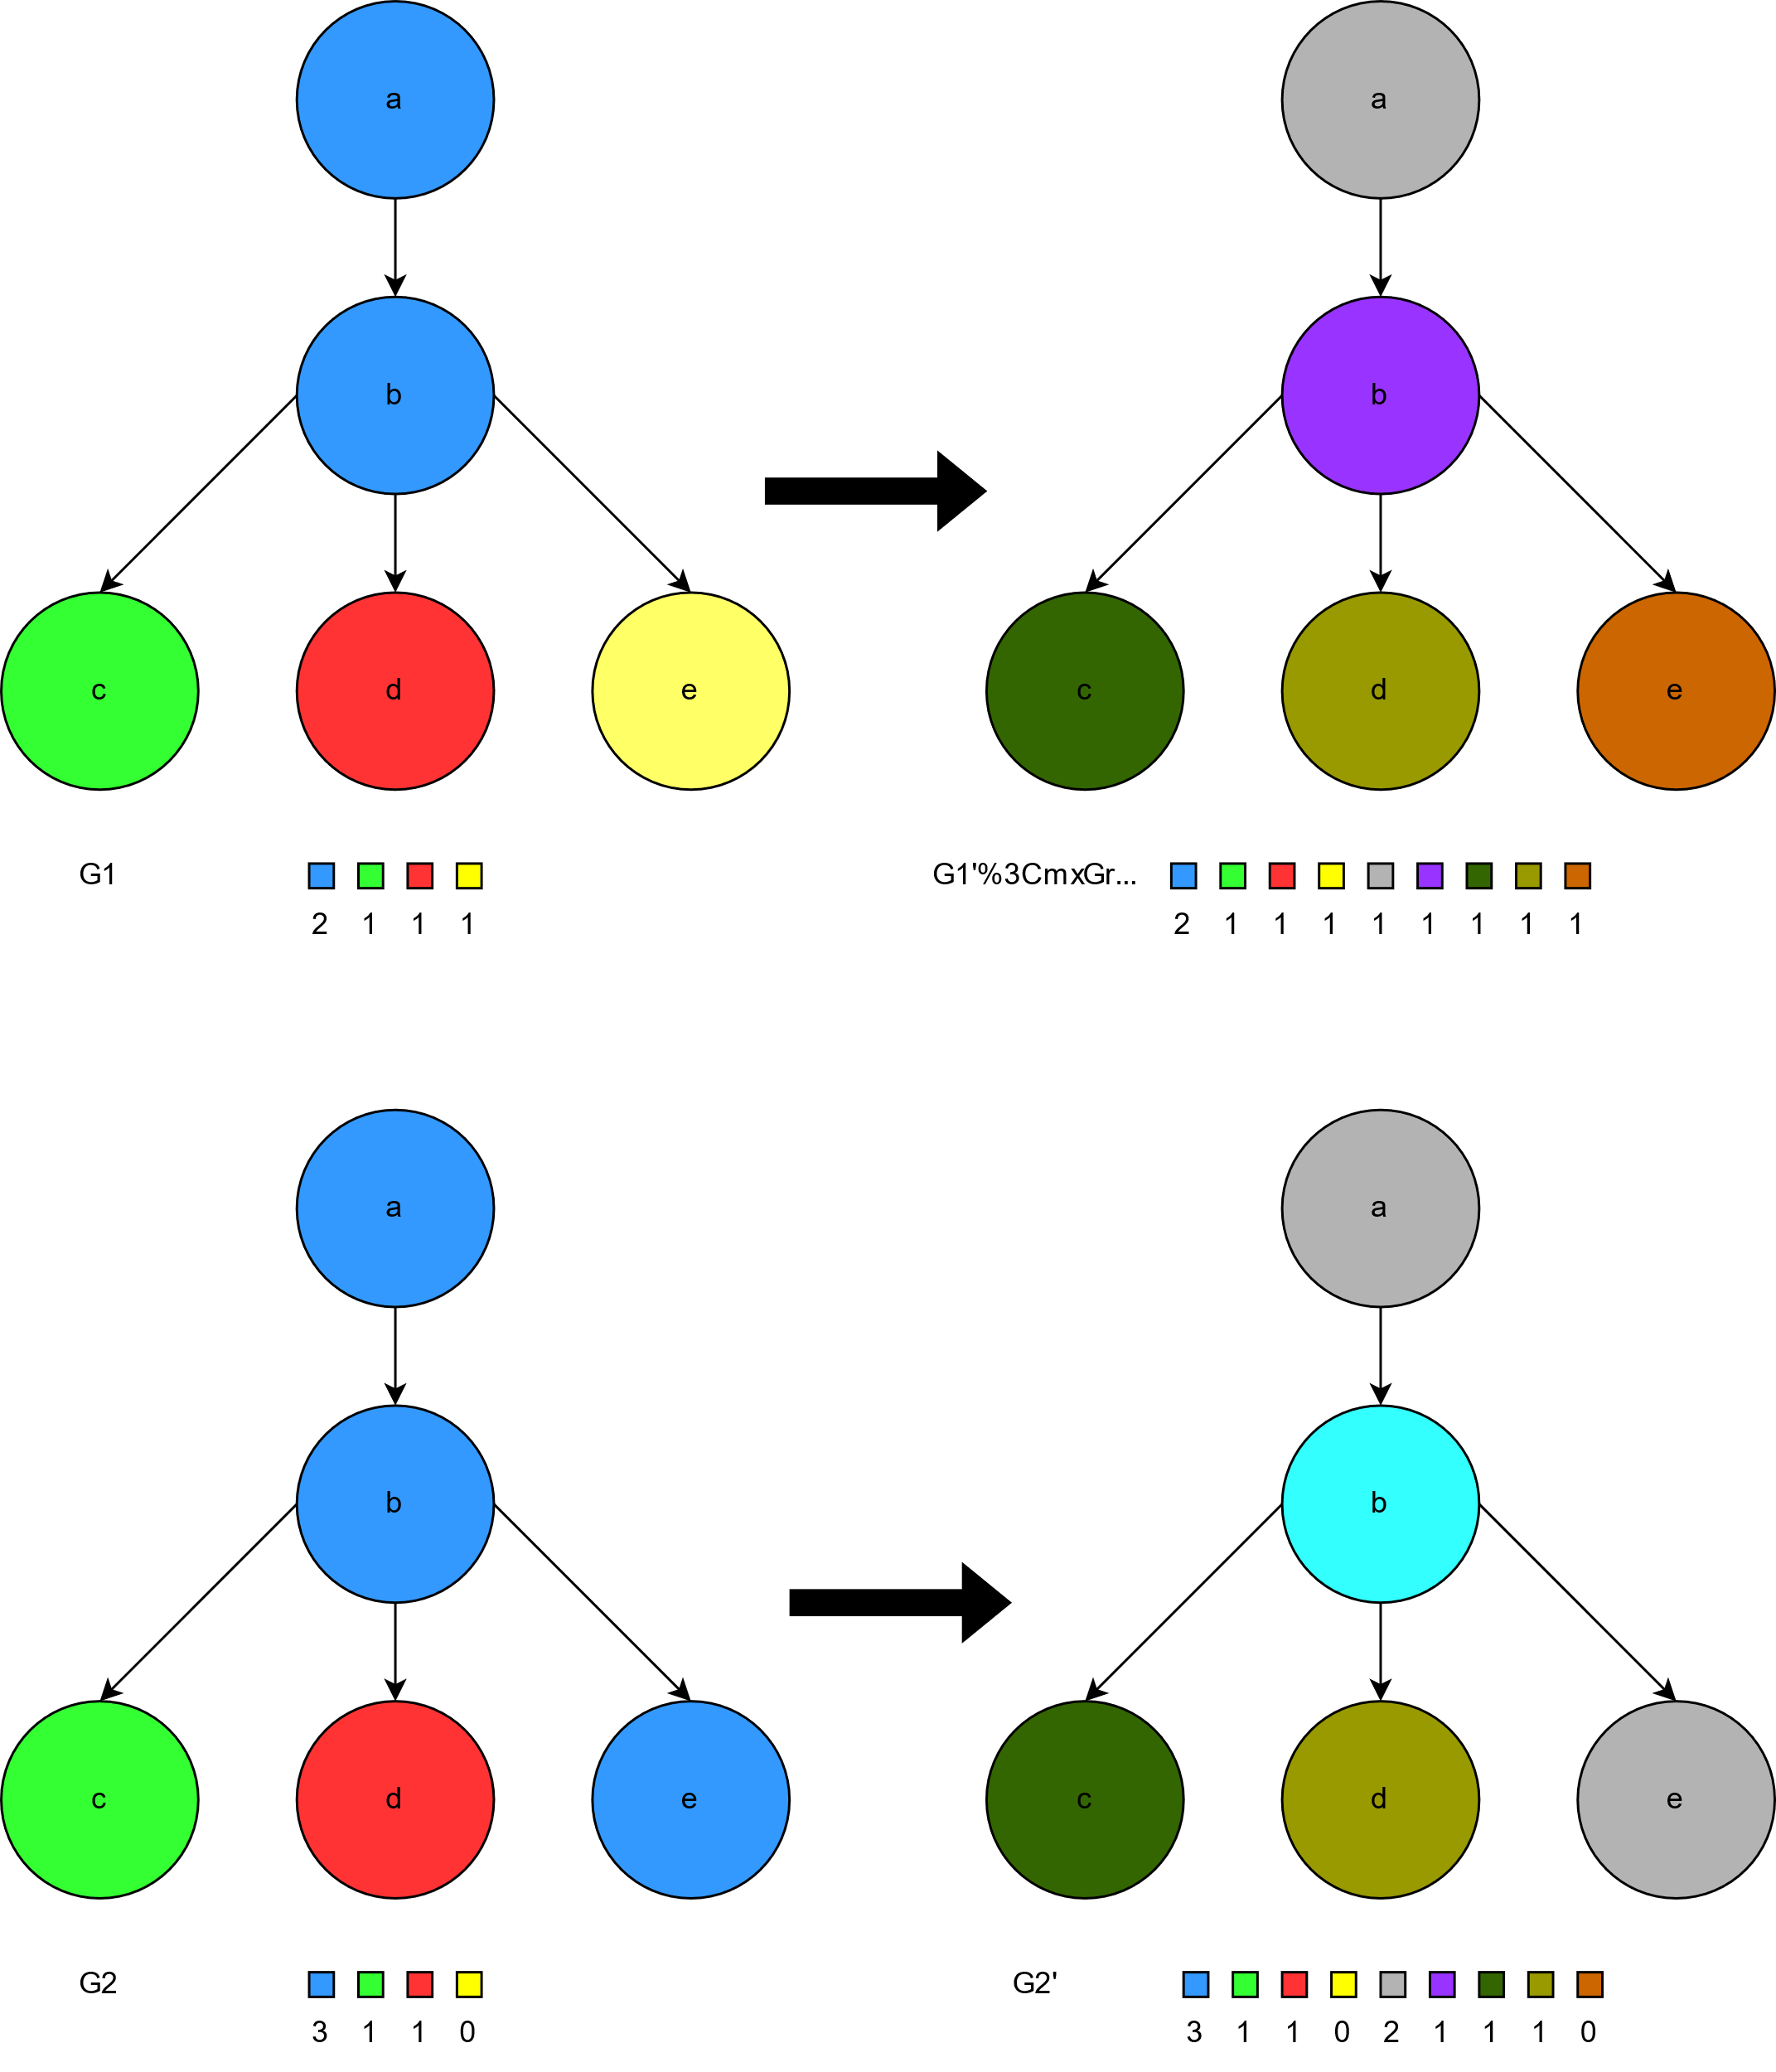
\includegraphics[width=0.5\textwidth,height=\textheight]{wl.png}

}

\caption{\label{fig-wl}One iteration of the WL kernel. Feature vectors
initially consist of counts of original node labels. At each iteration,
new labels (colors) are created for each atoms by considering the labels
of its neighbours. Nodes a in both G1' and G2' are labeled grey as they
were both adjacent to a single blue label in the previous iteration,
whereas nodes e in G1' and G2' are assigned different labels due to the
differences in their neighbouring node labels. The feature vectors
consist of counts of the original and newly created node labels as
iteration continues until a defined limit or convergence is reached. The
inner products are computed to obtain a similarity score.}

\end{figure}%

\subsubsection{Graph Embeddings}\label{sec-graphembed}

Whilst there are numerous advantageous qualities to graph
representations, the unstructured, relational nature of the data does
not allow it to be directly used as inputs into QSAR models which
require numerical data in the form of vectors
\citep{cai_comprehensive_2018}. To overcome this limitation, graph
embedding techniques are used to create lower dimensional
representations of graph data whilst retaining as much topological and
label (or feature) information as possible. Graph embeddings allow for a
type of similarity measurement between graphs. Embedding methods
represent graphs in a multi-dimensional latent space, where highly
similar molecular graphs will lie near each other, whereas dissimilar
molecular graphs will lie further apart. The distance between the
embedding of two molecular graphs in the latent space provides a
quantitative measure of similarity.

A number of different methods exist that are capable of creating graph
embeddings which can be broadly divided into two categories: node
embeddings, and whole graph embeddings. \textbf{Node embeddings} map
individual atoms in a molecular graph to numerical vectors, capturing
atom characteristics and relationships. \textbf{Graph embeddings} on the
other hand represent the entire molecular graph as a single vector,
often by combining atom embeddings or using other methods, to permit
pairwise molecular graph comparisons. There are a variety of different
approaches to either task, with well established taxonomies in
literature dividing them into three distinct categories; matrix
factorisation methods, random walk based methods, and neural network
methods, with substantial areas of overlap between the three
\citep{xu_understanding_2021, goyal_graph_2018}.

Matrix factorisation techniques were the earliest studied, beginning
with the multi-dimensional scaling (MDS) that decomposed adjacency
matrices \citep{RN34}. Other factorisation methods operate on graph
proximity (distance matrices) or graph Laplacian matrices
\citep{RN35, RN36}. Although factorisation methods are the most
well-established and theoretically understood, they often scale poorly
\citep{xu_understanding_2020}. Random walk based embeddings
\citep{perozzi_deepwalk_2014} later emerged based upon word and document
embedding methodologies such as Word2Vec, adopting the skip-gram neural
network model used to create word embeddings to the graph context. The
skip-gram model is a simple single hidden layer neural network (see
Figure~\ref{fig-skip}) that is trained to predict the probabilities for
each word in a given vocabulary to appear near in sequence to a given
target word. The network is trained, and the weights of the trained
network are exploited as vectorised word embeddings, with the underlying
intuition being that words that often appear in similar contexts are
likely highly similar in some context \citep{mikolov_efficient_2013}.

\begin{figure}

\centering{

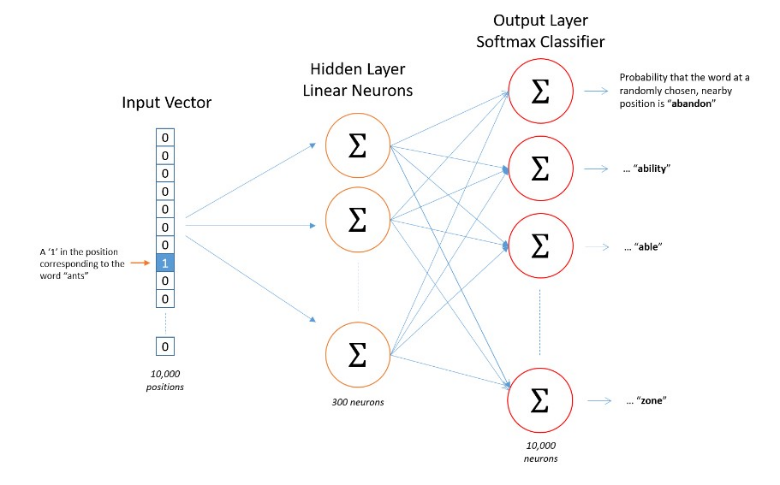
\includegraphics{survey_skip_gram_figure.png}

}

\caption{\label{fig-skip}Skip gram model for Word2Vec word embeddings. A
one hidden layer neural network is trained to determine the
probabilities for each word in a vocabulary of appearing near in
sequence to a given target word. The target word is given as a one-hot
encoded input, and after training via backpropagation over a number of
epochs, the hidden weights of the network are used as embedded vector
representations of words.}

\end{figure}%

In the chemistry domain, Jaeger et al \citep{jaeger_mol2vec_2018}
developed Mol2vec which is synonymous to the concept of Word2Vec.
Mol2Vec was developed to learn vector representations of molecular
substructures that point in similar directions for chemical related
substructures. Substuctures were derived using the the Morgan algorithms
as ``words'' and substances as ``sentences''. The Word2Vec algorithm was
then applied to a corpus of 19.9 million substances taken from the ZINC
and ChEMBL databases. The feature vectors for the substructures
generated were then summed to obtain substance vectors which could be
used as inputs for any subsequent machine learning approaches. Zhang et
al \citep{zhang_spvec_2019} proposed SPVec, constructed via the
combination of SMILES2Vec and ProtVec to represent specific drug-target
interactions, where the drug representation was simplified by using
SMILES directly.~Different from the work by Jaeger et al.
\citep{jaeger_mol2vec_2018}, SMILES of drug molecules were used directly
rather than generating Morgan substructures as ``words'' to learn the
representations. The approach described in Asgari and Mofrad
\citep{asgari_continuous_2015} was used to train ProtVec here, where
protein sequences were regarded as ``sentences'' and every three
non-overlapping amino acids were regarded as a ``word.'' SMILES2Vec
itself was developed by Goh et al \citep{goh_smiles2vec_2018} using a
deep recurrent neural network (RNN).

DeepWalk adapted the SkipGram approach to a graph setting
\citep{perozzi_deepwalk_2014} for node embedding. Words are analogous to
nodes in the graph, the sequences of words (a ``context'') are analogous
to random walks across node neighborhoods, and the vocabulary of words
is analogous to all nodes in the graph. Node2Vec iterated upon DeepWalk
with the introduction of parameters to control the length and freedom of
the random walk operations \citep{RN40}. Graph2Vec iterated upon
Node2Vec to allow for skip-gram based whole graph embeddings based off
rooted subgraphs analogous to words in Word2Vec
\citep{narayanan_graph2vec_2017}. In the context of molecular graphs,
Graph2Vec identifies recurring substructures across many molecules and
learns which are important and how they combine to form the whole
molecule. The information is then encoded into a fixed length vector for
each molecule. Each molecule is represented by a vector that captures
the overall structure from both a local perspective (in terms of
specific functional groups) in additional to more global patterns (like
the arrangement of these features). GL2Vec improved upon Graph2Vec in
classification tasks by incorporating information gleaned from a line
graph representation, better allowing for the capture of structural
information \citep{RN42}. Research has shown that more complicated
approaches to graph embeddings may not necessarily result in better
performance. The LDP (Local Degree Profile) embedding method was
introduced in 2019 and showed comparable performance to more
sophisticated embeddings methods while only considering the degree
information of nodes in a graph without considering any label
information whatsoever \citep{RN32}.

\subsubsection{Deep Learning Embeddings}\label{deep-learning-embeddings}

Graph neural networks (GNNs) were introduced in 2009 with the goal of
extending existing neural network models for processing graph structured
data \citep{scarselli_graph_2009}. Graph convolutional networks (GCNs)
were introduced by Duvenaud et al. \citep{duvenaud2015convolutional} to
operate on graphs for molecular property predictions. Subsequently,
Coley et al. \citep{coley2017convolutional} constructed feature vectors
of atoms using atom and bond attributes in molecules and considered
local chemical environment information within different neighborhood
radii. By directly inputting the complete molecular graph into CNN, the
model could learn to recognise atom cluster features, significantly
improving the performance of the CNN model. Gilmer et al.
\citep{gilmer2017international} reformulated existing models as message
passing neural networks (MPNN) and leveraged MPNN to demonstrate
state-of-the-art results on quantum mechanical property prediction tasks
for small organic molecules. Wang et al.~(2019) used graph structures
with convolutional networks to discover the relationship of each atom
and designed a convolution spatial graph embedding layer (C-SGEL) to
make full use of the spatial connectivity information of molecules
\citep{wang_molecule_2019}.

At the base level, GCNs take a graph as input and pass it through a
number of convolutional layers that aggregate each nodes neighbourhood
information. At each training epoch, each node in the graph has its
hidden state updated by aggregating each of the node's neighbours hidden
states together by some function and combining it with the current
hidden state of the node. The output of convolutional layers is a set of
node embeddings, vectorised representations of each node in the graph.
Whole graph embeddings are generated from these individual node
embeddings by combining them through a ``pooling'' layer that aggregates
the node embeddings together. The resulting embeddings can then be used
as inputs into different regression or classification based machine
learning models.

\begin{figure}

\centering{

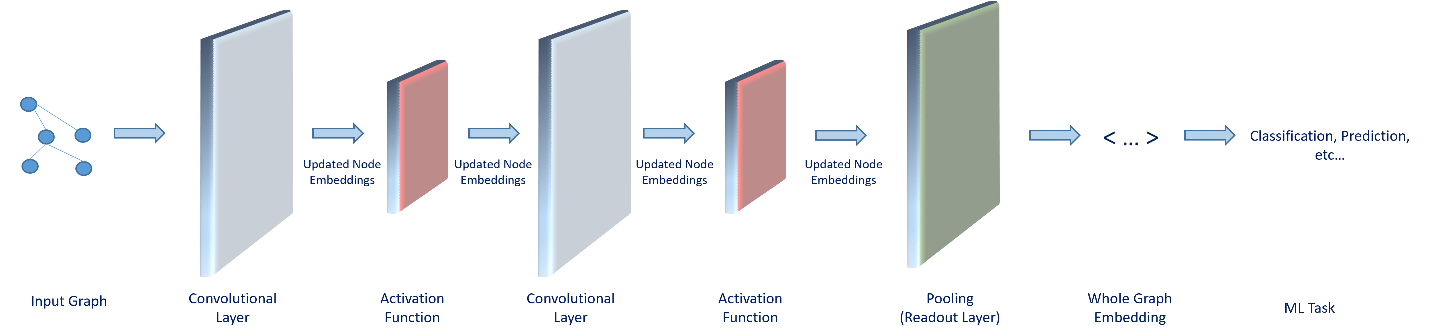
\includegraphics{gcn_model.png}

}

\caption{\label{fig-gcn-concept}Graph convolutional network conceptual
model. A graph is given as input into the model and passed through a
series of convolutional layers and activation functions that produce
embeddings for each node in the graph. The individual node embeddings
are aggregated together by some pooling operation in a readout layer in
order to produce a whole graph embedding as output that can be used for
structured ML tasks such as classification, regression, or prediction.}

\end{figure}%

The aim of this study was to compare and contrast different graph based
approaches and their utility in assessing similarity for read-across.
Morgan chemical and ToxPrint fingerprints were used as baseline
comparators. Five different datasets were used to explore the graph
kernel similarity, graph embedding, and deep learning (DL) approaches.
The datasets were varied in size from an analogue approach case at one
end of the spectrum to a larger dataset of genotoxicity outcomes for
several thousand substances. The selection of the datasets were
influenced by several considerations, namely they represented a range of
endpoints and use cases which could influence the use of molecular
similarity. For example, a single analogue approach would capture an
expert assessment use case for repeated dose toxicity which would rely
on finding a handful of candidate analogues with relevant data whereas
the genotoxicity dataset with a large number of substances could
leverage the potential utility of deep learning approaches.

\section{Methods}\label{methods}

\subsection{Datasets analysed}\label{datasets-analysed}

In total, five different datasets were chosen to investigate similarity
in this study. These datasets were chosen as they represented different
read-across scenarios, thus allowing several different types of
similarity calculations to be performed on different representations of
chemical structure. Table~\ref{tbl-datasets} summarises the datasets.

\begin{longtable}[]{@{}
  >{\centering\arraybackslash}p{(\columnwidth - 10\tabcolsep) * \real{0.1167}}
  >{\centering\arraybackslash}p{(\columnwidth - 10\tabcolsep) * \real{0.1833}}
  >{\centering\arraybackslash}p{(\columnwidth - 10\tabcolsep) * \real{0.1333}}
  >{\centering\arraybackslash}p{(\columnwidth - 10\tabcolsep) * \real{0.2833}}
  >{\centering\arraybackslash}p{(\columnwidth - 10\tabcolsep) * \real{0.1333}}
  >{\centering\arraybackslash}p{(\columnwidth - 10\tabcolsep) * \real{0.1500}}@{}}
\caption{The datasets investigated in this study with a description of
the coverage and scope.}\label{tbl-datasets}\tabularnewline
\toprule\noalign{}
\begin{minipage}[b]{\linewidth}\centering
Dataset No.
\end{minipage} & \begin{minipage}[b]{\linewidth}\centering
Effect/Toxicity
\end{minipage} & \begin{minipage}[b]{\linewidth}\centering
No.~Chemicals
\end{minipage} & \begin{minipage}[b]{\linewidth}\centering
Types of Chemicals
\end{minipage} & \begin{minipage}[b]{\linewidth}\centering
Techniques attempted
\end{minipage} & \begin{minipage}[b]{\linewidth}\centering
Reference
\end{minipage} \\
\midrule\noalign{}
\endfirsthead
\toprule\noalign{}
\begin{minipage}[b]{\linewidth}\centering
Dataset No.
\end{minipage} & \begin{minipage}[b]{\linewidth}\centering
Effect/Toxicity
\end{minipage} & \begin{minipage}[b]{\linewidth}\centering
No.~Chemicals
\end{minipage} & \begin{minipage}[b]{\linewidth}\centering
Types of Chemicals
\end{minipage} & \begin{minipage}[b]{\linewidth}\centering
Techniques attempted
\end{minipage} & \begin{minipage}[b]{\linewidth}\centering
Reference
\end{minipage} \\
\midrule\noalign{}
\endhead
\bottomrule\noalign{}
\endlastfoot
1 & Repeated dose toxicity & 6 & Analogue approach for a nitrotoluene
and its analogues & WL & \href{https://www.epa.gov/pprtv}{PPRTV} \\
2 & Local Lymph Node Assay (LLNA) for skin sensitisation that have both
chemical and biological diversity & 222 & A broad range of chemicals
capturing different reactivity mechanisms & WL, Graph2Vec, Mol2Vec &
Patlewicz et al \citep{patlewicz_can_2016}; Asturiol et al
\citep{asturiol_consensus_2016} \\
3 & Fathead Minnow MOA aquatic acute toxicity & 617 & Broad range of
chemicals capturing different MOAs & WL, Graph2Vec, Mol2Vec &
\href{https://sourceforge.net/projects/toxmatch/}{Dataset taken from
ToxMatch} \\
4 & BfR skin irritation & 70 & Training set of chemicals including
aliphatic alcohols, esters, aldehydes and haloalkanes with
classification information for skin irritation that was used to inform
the BfR rulebase & WL &
\href{https://toxtree.sourceforge.net/skin.html}{Dataset taken from
Toxtree} \\
5 & Genotoxicity dataset & 5403 & Summary genotoxicity outcomes
extracted from ToxValDB 9.5 but aggregated in accordance with
\citep{pradeep_evaluation_2021} & Graph2Vec, GCN & Pradeep et al.
\citep{pradeep_evaluation_2021} \\
\end{longtable}

\subsection{Chemical representations}\label{chemical-representations}

Morgan chemical fingerprints were generated using a radius of 3 and a
bitvector length of 2048. ToxPrints were the original 729 features
described in Yang et al. \citep{yang_new_2015}. The WL substree kernel
were generated using the Grakel python
library\citep{siglidis_grakel_2020}. Node level information used for the
derivation of WL kernels comprised the atom type, its degree,
hybridisation, aromaticity, formal charge and implicit hydrogen count.
Graph2Vec embeddings were created using the KarateClub
package\citep{karateclub} from which pairwise cosine distances were
calculated. Word2Vec was used to derive a model based on tokenised
Morgan fingerprints to derive Mol2Vec type embeddings. A Mol2Vec
approach to learning molecular embeddings inspired by natural language
processing techniques like Word2Vec was applied to train a model to
uncover embeddings. The DSSTox library of approx 0.5 million discrete
structures was used as a corpus of diverse chemicals. SMILES were
tokenised on the basis of Morgan chemical fingerprints. Gensim's
\citep{rehurek2011gensim} Word2Vec engine to used to train a model to
learn embeddings for the molecular fragments. Embeddings for the entire
molecule were created by taking the mean of the fragment embeddings.

The performance of the different representations were analysed via
visualisation of the similarity (or distance) matrices. The ranges of
scores were summarised as ranges to determine if any insights could be
derived as to whether certain representations worked better for
different datasets studied.

For the largest dataset, genotoxicity, the Graph2Vec embeddings were
also used as inputs in two classifier models; a k-NN classifier and
logistic regression to assess their informative content. The 2
classifiers were implemented using the open source Python package
scikit-learn \citep{RN53} with the area under the curve-receiver
operating characteristic (AUC-ROC) as a performance metric. Model
performance was assessed through a 5-fold cross validation procedure.

For the deep learning graph convolutional neural network model, three
convolutional layers (GATv2Conv convolutional layer, a graph attentional
layer from Brody et al. \citep{RN56} with ReLU activation functions, a
global mean pooling readout layer, and a single fully connected linear
layer was used to make predictions. For the molecular graphs, one hot
encodings of the atom symbol labels were attached as node feature
vectors. The graphs were split into a training and validation set. Using
cross entropy loss and an Adam optimiser with a learning rate of 0.001,
the model was trained over 50 epochs, with the AUC score of the training
and validation graphs reported at each epoch. After training, embeddings
for the validation graphs were generated by inputting the graphs into
the trained model and extracting the resultant embedding from the
readout layer. These were visualised via t-SNE
\citep{van_er_maaten_visualizing_2018} and labelled by outcome. The
embeddings were also used as inputs into K-NN and logistic regression
classification models, with performance compared against the use of
Morgan chemical fingerprints.

\section{Data and code availability}\label{data-and-code-availability}

All analysis was performed in Python 3.10 using Jupyter notebooks. RDKit
was used for generation of Morgan chemical fingerprints. The EPA
Cheminformatics Modules were used to generate ToxPrints. Molecular graph
representations were created using the Python package RDKit
\citep{landrum_rdkit}. The open source Python package GraKeL
\citep{siglidis_grakel_2020} was used to implement the WL subtree
kernel. The open source Python package KarateClub was used to create the
Graph2Vec embeddings. Gensim \citep{rehurek2011gensim} was used to train
the Word2Vec model for the Mol2Vec approach. Scikit-learn \citep{RN53}
was used to develop k-NN and logistic models for the embeddings derived
from the Graph2Vec and GCN approaches. Pytorch geometric
\citep{fey2019fastgraphrepresentationlearning} was used to train a GCN
model for the genotoxicity dataset.

\section{Results and Discussion}\label{results-and-discussion}

\subsection{Pairwise similarities}\label{pairwise-similarities}

\subsubsection{LLNA}\label{sec-llna}

The LLNA dataset comprised 222 substances with their associated skin
sensitising outcome as well as their reaction chemistry domain which
discriminated between sensitisers that might act by a Schiff base
mechanism from a Michael acceptor mechanism. The five main reaction
domains associated with skin sensitisation are described by Roberts and
Aptula in 2008 \citep{roberts_determinants_2008}. Essentially, the rate
determining step for skin sensitisation relies on a substance forming a
covalent bond with a skin protein, thus substances that are
electrophilic in nature can bind with nucleophilic skin proteins.
Identifying potential skin sensitisers tends to involve identifying
electrophilic reaction sites e.g.~substances such as alpha,
beta-unsaturated esters or aldehydes are activated to be able to act via
a Michael addition reaction.

Pairwise Jaccard similarities calculated from using Morgan chemical
fingerprints were found to be typically low across the entire LLNA
dataset. The maximum of the median pairwise similarities across all he
substances was only 0.125, whereas the minimum value was 0.021. This
marginally increased when the dataset was filtered to consider a
specific reaction domain - the range of median pairwise similarities
across the 29 Michael acceptors was 0.04-0.16, for the 20 Schiff base
formers this was 0.05-0.13 and for the 14 Acyl transfer agents, it was
0.06-0.16. Pairwise Jaccard similarities across ToxPrints were higher,
with the maximum median Jaccard similarity being 0.17 for the entire
dataset but higher values were found for specific reaction domains; for
Michael acceptors the maximum median Jaccard similarity was 0.32, for
Schiff base formers, 0.25 and Acyl transfer agents was 0.195. Maximum
median pairwise similarities were even higher using the WL subtree
kernel; 0.34 for the entire dataset whereas the values tended to be
lower for specific reaction domains e.g.~0.24 for Michael acceptors,
0.22 for Schiff base formers and 0.34 for Acyl transfer agents.

Figure~\ref{fig-ma} shows the pairwise similarities for the Michael
acceptors using all 3 approaches where the orange cells are indicative
of higher pairwise similarities. In panel 3 of Figure~\ref{fig-ma}, few
pairs of substances appear to be very similar based on Morgan
fingerprints whereas there is a greater number within the WL and
ToxPrint pairwise comparisons. For Michael acceptors characterised by
Morgan fingerprints, 49\% of the pairwise comparisons had similarities
ranging from 0-0.1 whereas 43\% of the comparisons fell within a
similarity range of 0.1-0.3. In contrast, across the whole dataset
characterised by Morgan fingerprints, 71\% of the pairwise comparisons
had a Jaccard similarity range of 0-0.1, with 27\% having a similarity
range of 0.1-0.3. For ToxPrints within the Michael acceptor domain, the
variation was very different with 30\% having a Jaccard similarity range
between 0-0.1, 43\% with a Jaccard similarity range of 0.1-0.3, 20\%
having a Jaccard similarity range of 0.3-0.5, and the remainder with
similarities in excess of 0.5. Approx 5\% of WL scores within the
Michael domain were greater than 0.5.

\begin{longtable}[]{@{}cccccc@{}}
\caption{Percentage of Michael acceptor pairs that fall into different
similarity thresholds based on their structural
representation}\tabularnewline
\toprule\noalign{}
Fingerprint Representation & 0-0.1 & 0.1-0.3 & 0.3-0.5 & 0.5-0.7 &
0.7-1 \\
\midrule\noalign{}
\endfirsthead
\toprule\noalign{}
Fingerprint Representation & 0-0.1 & 0.1-0.3 & 0.3-0.5 & 0.5-0.7 &
0.7-1 \\
\midrule\noalign{}
\endhead
\bottomrule\noalign{}
\endlastfoot
Morgan & 49\% & 43.6\% & 6.6\% & 0.2\% & 0.2\% \\
ToxPrint & 30.5\% & 43\% & 19.9\% & 4.67\% & 1.7\% \\
WL & 31\% & 52.2\% & 11.8\% & 4.4\% & 0.4\% \\
\end{longtable}

\begin{figure}

\centering{

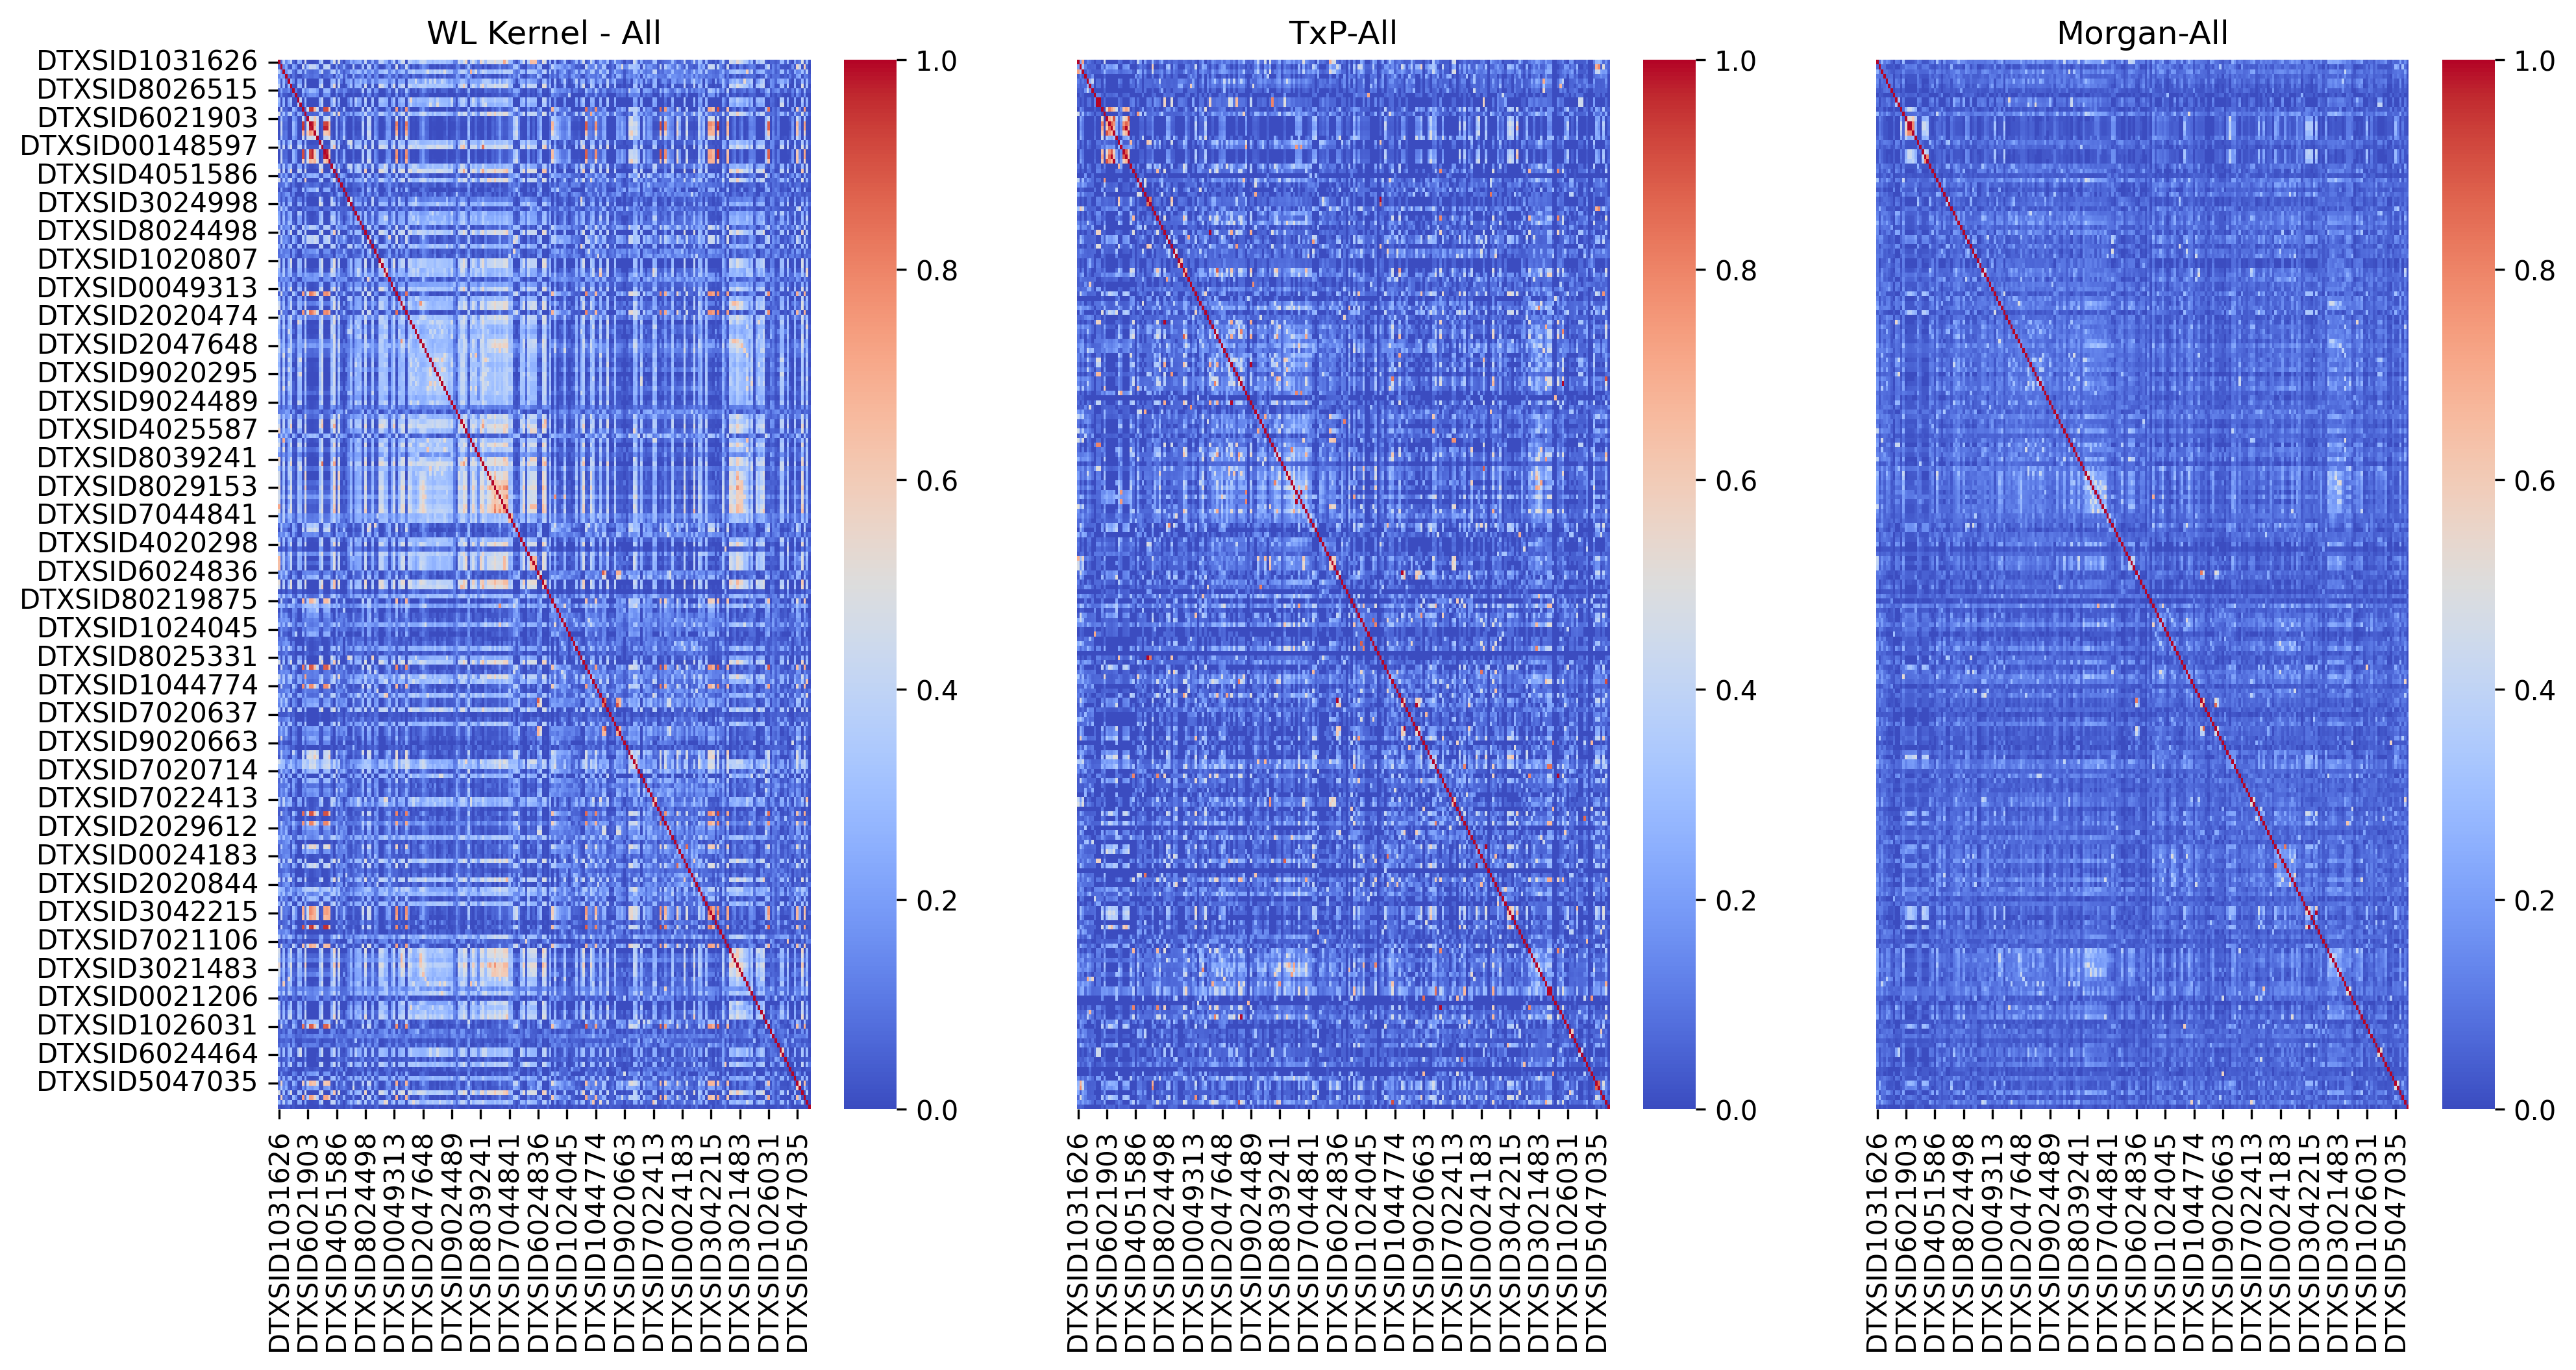
\includegraphics{llna_sim_all.png}

}

\caption{\label{fig-ma}Pairwise similarity matrices across the 3
approaches for Michael acceptors. The pockets of oranges throughout the
matrix highlight those pairs of chemicals that are most similar to each
other. The frequency of the orange squares is much more pronounced in
the ToxPrints heatmap overall whereas there are few if any cases in the
Morgan heatmap.}

\end{figure}%

\begin{figure}[H]

{\centering 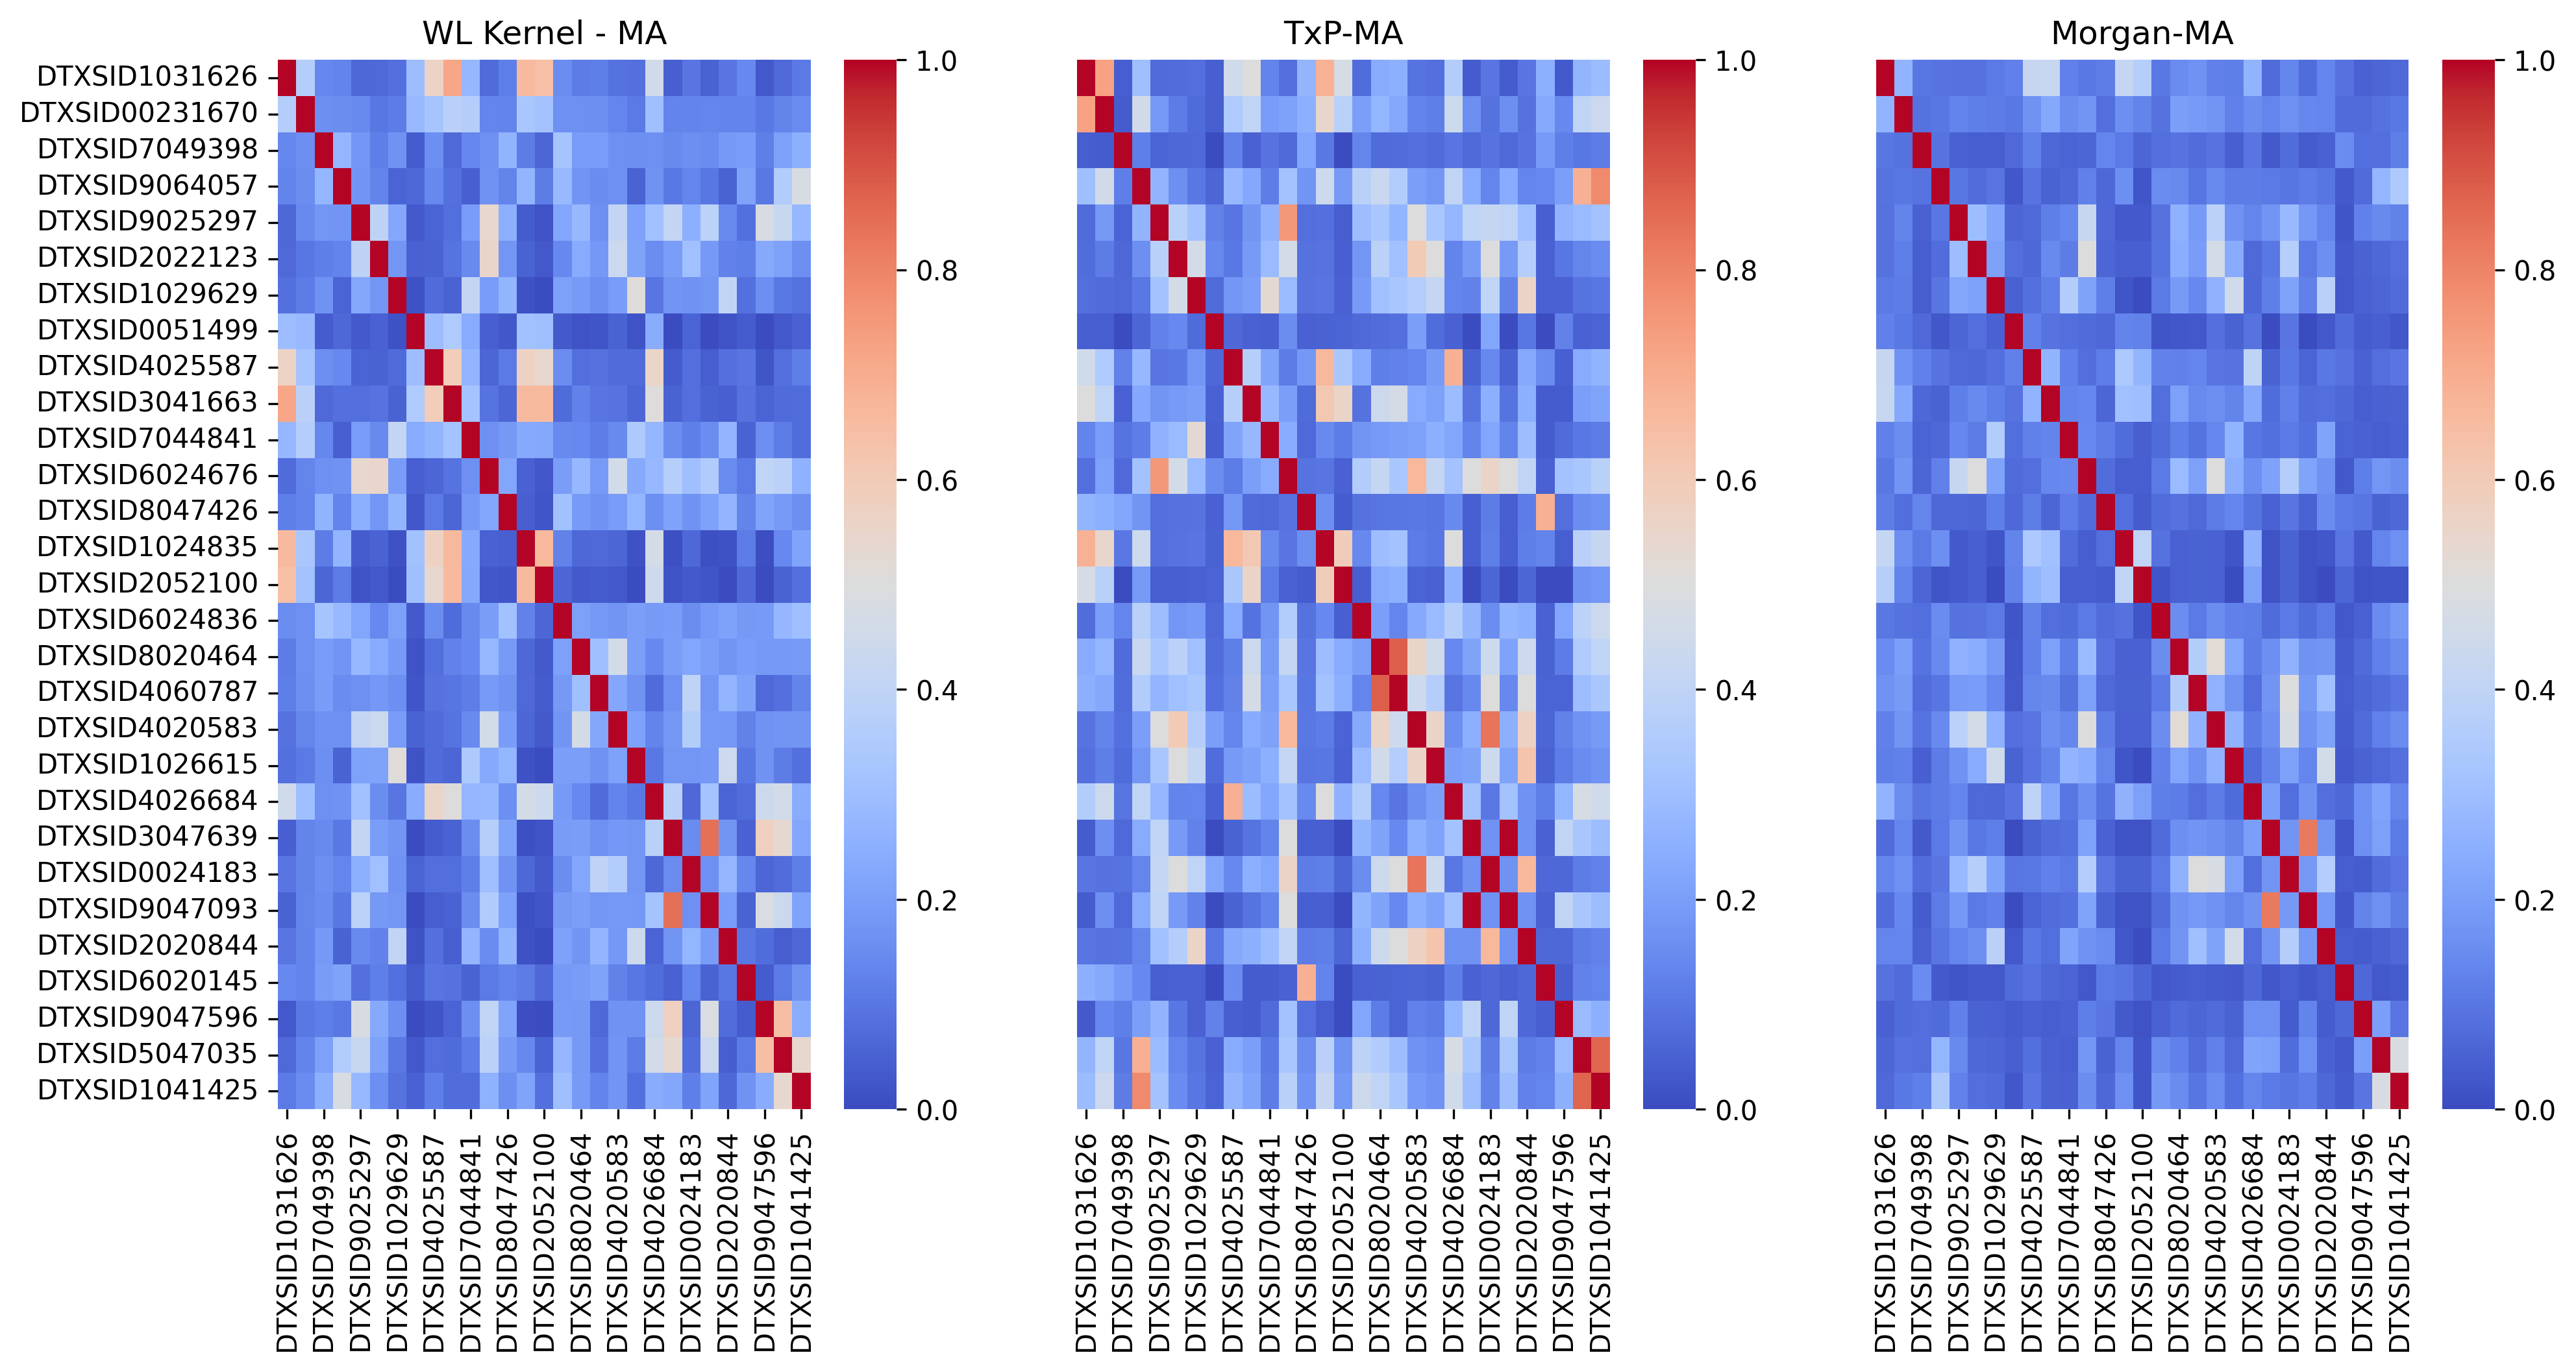
\includegraphics{llna_sim_MA.png}

}

\caption{Pairwise similarity matrices for Michael acceptors}

\end{figure}%

There would be an expectation of greater pairwise similarity within a
given reaction domain, as the scope of the chemicals would be expected
to react via the same reaction chemistry. The fact that the WL and
ToxPrints showed a higher proportion of more similar pairs indicates
that both these representations appear to be able to better capture the
features important for the chemistry of the reaction domain. In
contrast, there was little to discriminate the substances when
represented by Morgan chemical fingerprints as indicated by the large
proportion of pairwise similarities falling in the lowest ranges.
Indeed, ToxPrints captured structural features that characterised the
reaction domains well which explains the greater proportion of higher
pairwise similarities. The WL approach appeared to be often better at
characterising substructural features relevant for skin sensitisation
better than Morgan fingerprints, as evidenced by almost 5\% of pairs
have a similarity of 0.5 or greater contrasted with only 0.4\% of pairs
based on Morgan fingerprints. A handful of example pairs from the same
reaction are shown in Table~\ref{tbl-rxnss} which demonstrates the
higher similarities when using ToxPrints and the WL kernel.

\begin{longtable}[]{@{}
  >{\centering\arraybackslash}p{(\columnwidth - 10\tabcolsep) * \real{0.0984}}
  >{\centering\arraybackslash}p{(\columnwidth - 10\tabcolsep) * \real{0.2951}}
  >{\centering\arraybackslash}p{(\columnwidth - 10\tabcolsep) * \real{0.3115}}
  >{\centering\arraybackslash}p{(\columnwidth - 10\tabcolsep) * \real{0.0984}}
  >{\centering\arraybackslash}p{(\columnwidth - 10\tabcolsep) * \real{0.0984}}
  >{\centering\arraybackslash}p{(\columnwidth - 10\tabcolsep) * \real{0.0984}}@{}}
\caption{Example cases of substances sharing the same reaction domain
and their associated pairwise similarity
score}\label{tbl-rxnss}\tabularnewline
\toprule\noalign{}
\begin{minipage}[b]{\linewidth}\centering
Domain
\end{minipage} & \begin{minipage}[b]{\linewidth}\centering
\end{minipage} & \begin{minipage}[b]{\linewidth}\centering
\end{minipage} & \begin{minipage}[b]{\linewidth}\centering
WL
\end{minipage} & \begin{minipage}[b]{\linewidth}\centering
TxP
\end{minipage} & \begin{minipage}[b]{\linewidth}\centering
Morgan
\end{minipage} \\
\midrule\noalign{}
\endfirsthead
\toprule\noalign{}
\begin{minipage}[b]{\linewidth}\centering
Domain
\end{minipage} & \begin{minipage}[b]{\linewidth}\centering
\end{minipage} & \begin{minipage}[b]{\linewidth}\centering
\end{minipage} & \begin{minipage}[b]{\linewidth}\centering
WL
\end{minipage} & \begin{minipage}[b]{\linewidth}\centering
TxP
\end{minipage} & \begin{minipage}[b]{\linewidth}\centering
Morgan
\end{minipage} \\
\midrule\noalign{}
\endhead
\bottomrule\noalign{}
\endlastfoot
SB & 2,2,6,6-Tetramethyl-3,5-heptanedione (DTXSID7049396) &
5-Methyl-2,3-hexanedione (DTXSID7049215) & 0.21 & 0.5 & 0.185 \\
MA & Ethyl acrylate (DTXSID4020583) & Butyl acrylate (DTXSID6024676) &
0.458 & 0.66 & 0.5 \\
MA & trans-2-decenal (DTXSID5047035) & trans-2-hexenal (DTXSID1041425) &
0.53 & 0.86 & 0.48 \\
Acyl & Phthalic anhydride (DTXSID2021159) & Trimellitic anhydride
(DTXSID7026235) & 0.538 & 0.7 & 0.368 \\
\end{longtable}

\subsubsection{BfR skin irritation}\label{bfr-skin-irritation}

The BfR dataset comprised 70 substances with their associated skin
irritation classification outcome per the former EU Classification and
Labelling regulation. Substances classified as irritants were labelled
with as R38. Figure~\ref{fig-bfr} shows heatmaps of the pairwise
similarities based on Morgan, ToxPrint and WL structural
representations. Overall, the WL heatmap shows a larger number of
similar pairings compared with the other 2 fingerprint types.

\begin{longtable}[]{@{}cccccc@{}}
\caption{Percentage of substance pairs that fall into different
similarity thresholds based on their structural
representation}\tabularnewline
\toprule\noalign{}
Fingerprint Representation & 0-0.1 & 0.1-0.3 & 0.3-0.5 & 0.5-0.7 &
0.7-1 \\
\midrule\noalign{}
\endfirsthead
\toprule\noalign{}
Fingerprint Representation & 0-0.1 & 0.1-0.3 & 0.3-0.5 & 0.5-0.7 &
0.7-1 \\
\midrule\noalign{}
\endhead
\bottomrule\noalign{}
\endlastfoot
Morgan & 74\% & 22\% & 2.98\% & 0.6\% & 0.2\% \\
ToxPrint & 65.9\% & 23.36\% & 8.29\% & 1.36\% & 0.9\% \\
WL & 49.8\% & 32.8\% & 9.8\% & 5.1\% & 2.3\% \\
\end{longtable}

\begin{figure}

\centering{

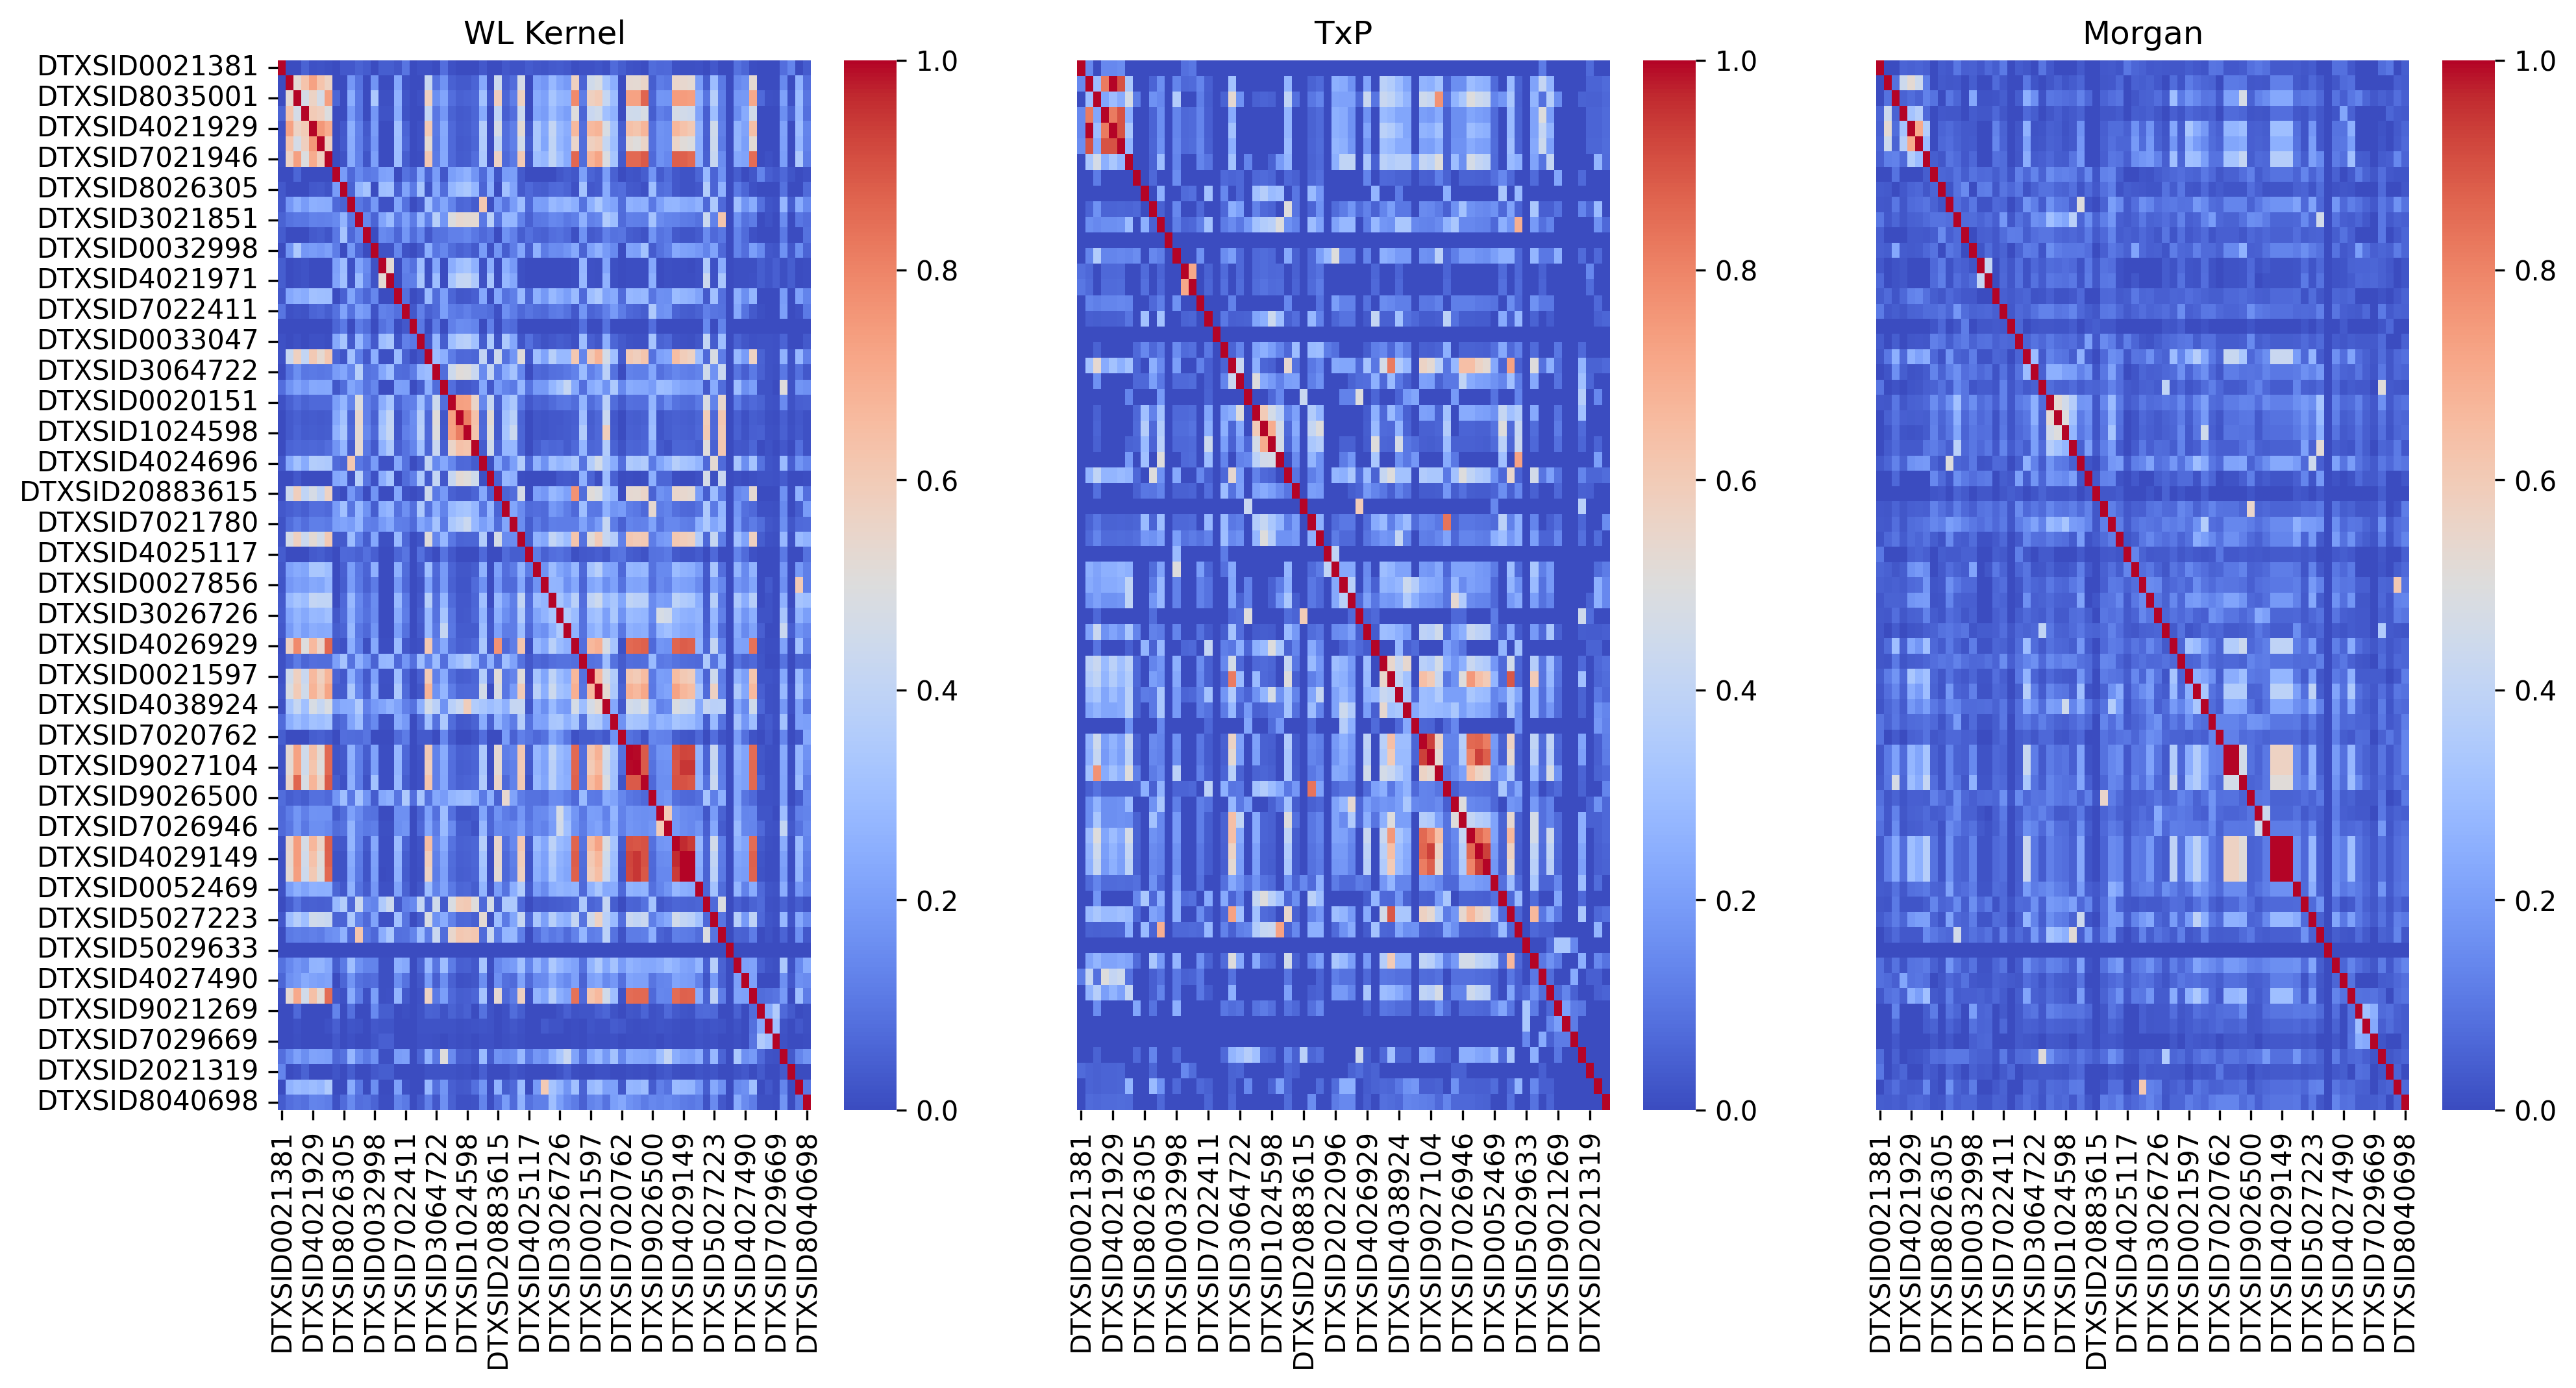
\includegraphics{bfr_sim.png}

}

\caption{\label{fig-bfr}Pairwise similarity matrices across the 3
approaches for the BfR dataset. The pockets of oranges throughout the
matrix highlight those pairs of chemicals that are most similar to each
other. The frequency of the orange squares is much more pronounced in
the WL heatmap overall whereas there are few if any cases in the Morgan
heatmap}

\end{figure}%

Table~\ref{tbl-bfrss} highlights several example pairs of chemicals and
their pairwise similarities. It is evident that ToxPrints are not able
to discriminate between the number of substituents present, such that
1,6-dibromohexane and 1-Bromohexane are considered equivalent whereas WL
gives rise to a high similarity but the similarity based on Morgan
fingerprints is only modest. The difference in chain length between
1-bromohexane and 1-bromopentane yields a much higher similarity when
using ToxPrints but is less pronounced for the other two
representations. Interestingly 1,6-dibromohexane is not irritating
whereas both 1-bromohexane and 1-bromopentane are classified as
irritating. None of the approaches take into account molecular size
attributes which may have modulated the differences in irritation
potential observed. 3-Phenylprop-2-enal and cyclamen aldehyde are both
aldehydes which share a benzene though one has the potential to react
through its double bond which is conjugated with the benzene ring. Both
are irritating but their pairwise similarities were low ranging from
0.125-0.274. alpha-Terpineol and D-Limonene share a cyclic diene
scaffold and are both irritating but their pairwise similarities are low
although consistent across the 3 representations (0.4-0.5).

\begin{longtable}[]{@{}
  >{\centering\arraybackslash}p{(\columnwidth - 8\tabcolsep) * \real{0.3385}}
  >{\centering\arraybackslash}p{(\columnwidth - 8\tabcolsep) * \real{0.4000}}
  >{\centering\arraybackslash}p{(\columnwidth - 8\tabcolsep) * \real{0.0769}}
  >{\centering\arraybackslash}p{(\columnwidth - 8\tabcolsep) * \real{0.0923}}
  >{\centering\arraybackslash}p{(\columnwidth - 8\tabcolsep) * \real{0.0923}}@{}}
\caption{Example cases of substances and their associated pairwise
similarity score}\label{tbl-bfrss}\tabularnewline
\toprule\noalign{}
\begin{minipage}[b]{\linewidth}\centering
\end{minipage} & \begin{minipage}[b]{\linewidth}\centering
\end{minipage} & \begin{minipage}[b]{\linewidth}\centering
WL
\end{minipage} & \begin{minipage}[b]{\linewidth}\centering
TxP
\end{minipage} & \begin{minipage}[b]{\linewidth}\centering
Morgan
\end{minipage} \\
\midrule\noalign{}
\endfirsthead
\toprule\noalign{}
\begin{minipage}[b]{\linewidth}\centering
\end{minipage} & \begin{minipage}[b]{\linewidth}\centering
\end{minipage} & \begin{minipage}[b]{\linewidth}\centering
WL
\end{minipage} & \begin{minipage}[b]{\linewidth}\centering
TxP
\end{minipage} & \begin{minipage}[b]{\linewidth}\centering
Morgan
\end{minipage} \\
\midrule\noalign{}
\endhead
\bottomrule\noalign{}
\endlastfoot
1,6-Dibromohexane (DTXSID4044452) & 1-Bromohexane (DTXSID4021929) & 0.72
& 1 & 0.52 \\
1-Bromohexane (DTXSID4021929) & 1-Bromopentane(DTXSID3049203) & 0.75 &
0.9 & 0.71 \\
3-Phenylprop-2-enal (DTXSID1024835) & Cyclamen aldehyde (DTXSID2044769)
& 0.27 & 0.2 & 0.13 \\
alpha-Terpineol (DTXSID5026625) & D-Limonene (DTXSID1020778) & 0.415 &
0.5 & 0.4 \\
\end{longtable}

When the pairwise similarities were stratified by whether substances
were irritants or not, with Morgan fingerprints, there was an increase
in the percentage pairs which were most similar (0.7-1) c.f 0.6\%
vs.~0.2\% whereas for ToxPrints, there was a shift for pairs with a low
similarity (0.3-0.5) c.f. 13\% vs 8.6\% and for WL, this shift was most
pronounced for moderate similarity range (0.5-0.7) cf.~7.69\% vs.~5.1\%.

Examples of irritants with the highest similarities between each other
were Sodium dodecyl sulfate (DTXSID1026031), Methyl hexadecanoate
(DTXSID4029149), 1-Decanol (DTXSID7021946), 10-Undecenoic acid
(DTXSID8035001), 1-Bromopentane (DTXSID3049203). However if a query was
performed for one of these e.g.~10-Undecenoic acid (DTXSID8035001), the
top 3 closest analogues (Dodecanoic acid (DTXSID5021590), Methyl
dodecanoate (DTXSID5026889), Methyl hexadecanoate (DTXSID4029149)) based
on their WL scores were noted to be structurally related but spanned
both irritants and non-irritants. None of the fingerprints used here
encodes any features that helps to discriminate for irritation
potential.

\subsubsection{Fathead Minnow (FHM)}\label{sec-fhm}

The FHM dataset comprised 617 substances with their associated acute
lethality outcomes in fathead minnow as well as their mode of action
(MOA) annotations. Probably the best known MOA scheme is that proposed
by Verhaaret al\citep{verhaar_1992}. The Verhaar scheme classifies
organic compounds into one of four categories: inert chemicals (Class
1), less inert chemicals (Class 2), reactive chemicals (Class 3), and
chemicals acting by a specific mechanism (Class 4). Chemicals in Class 1
exhibit nonpolar narcosis or baseline toxicity and can only be predicted
if they have log octanol:water partition coefficient (Kow) values
between 0 and 6 (e.g., benzenes).

Chemicals in Class 2 are more toxic and cause polar narcosis, and
typically possess hydrogen bond donor acidity (e.g., phenols and
anilines). Chemicals in Class 3 demonstrate enhanced toxicity as
compared to baseline toxicity and react nonspecifically with
biomolecules (e.g., epoxides) or are metabolised into more toxic species
(e.g., nitriles). Chemicals in Class 4 cause toxicity through a specific
mechanism such as acetylcholinesterase (AChE) inhibition by carbamate
insecticides. The assignment of a chemical to a class is based on a
decision tree that utilises the presence or absence of certain chemical
structures and moieties.

Pairwise similarities using Morgan, ToxPrint fingerprints and the WL
kernel were performed and stratified based on 2 of the MOAs (baseline
narcosis which had the highest number of chemicals and a specific MOA
for acetylcholinesterase activity (AChE)). Figure~\ref{fig-fhm} depicts
the heatmaps of the pairwise similarities based on these 3 structural
representations and 2 MOAs. Overall, the WL heatmap shows a large number
of similar pairings compared with the other 2 fingerprint types for
baseline narcotics (12\% of pairs had a similarity between 0.3-0.5)
whereas ToxPrints appear to better differentiate for AChEs (over 7\% of
pairs had a similarity greater than 0.5). In the latter case, this was
limited to several substances that were either closely related
carbamates or organophosphates.

\begin{figure}

\centering{

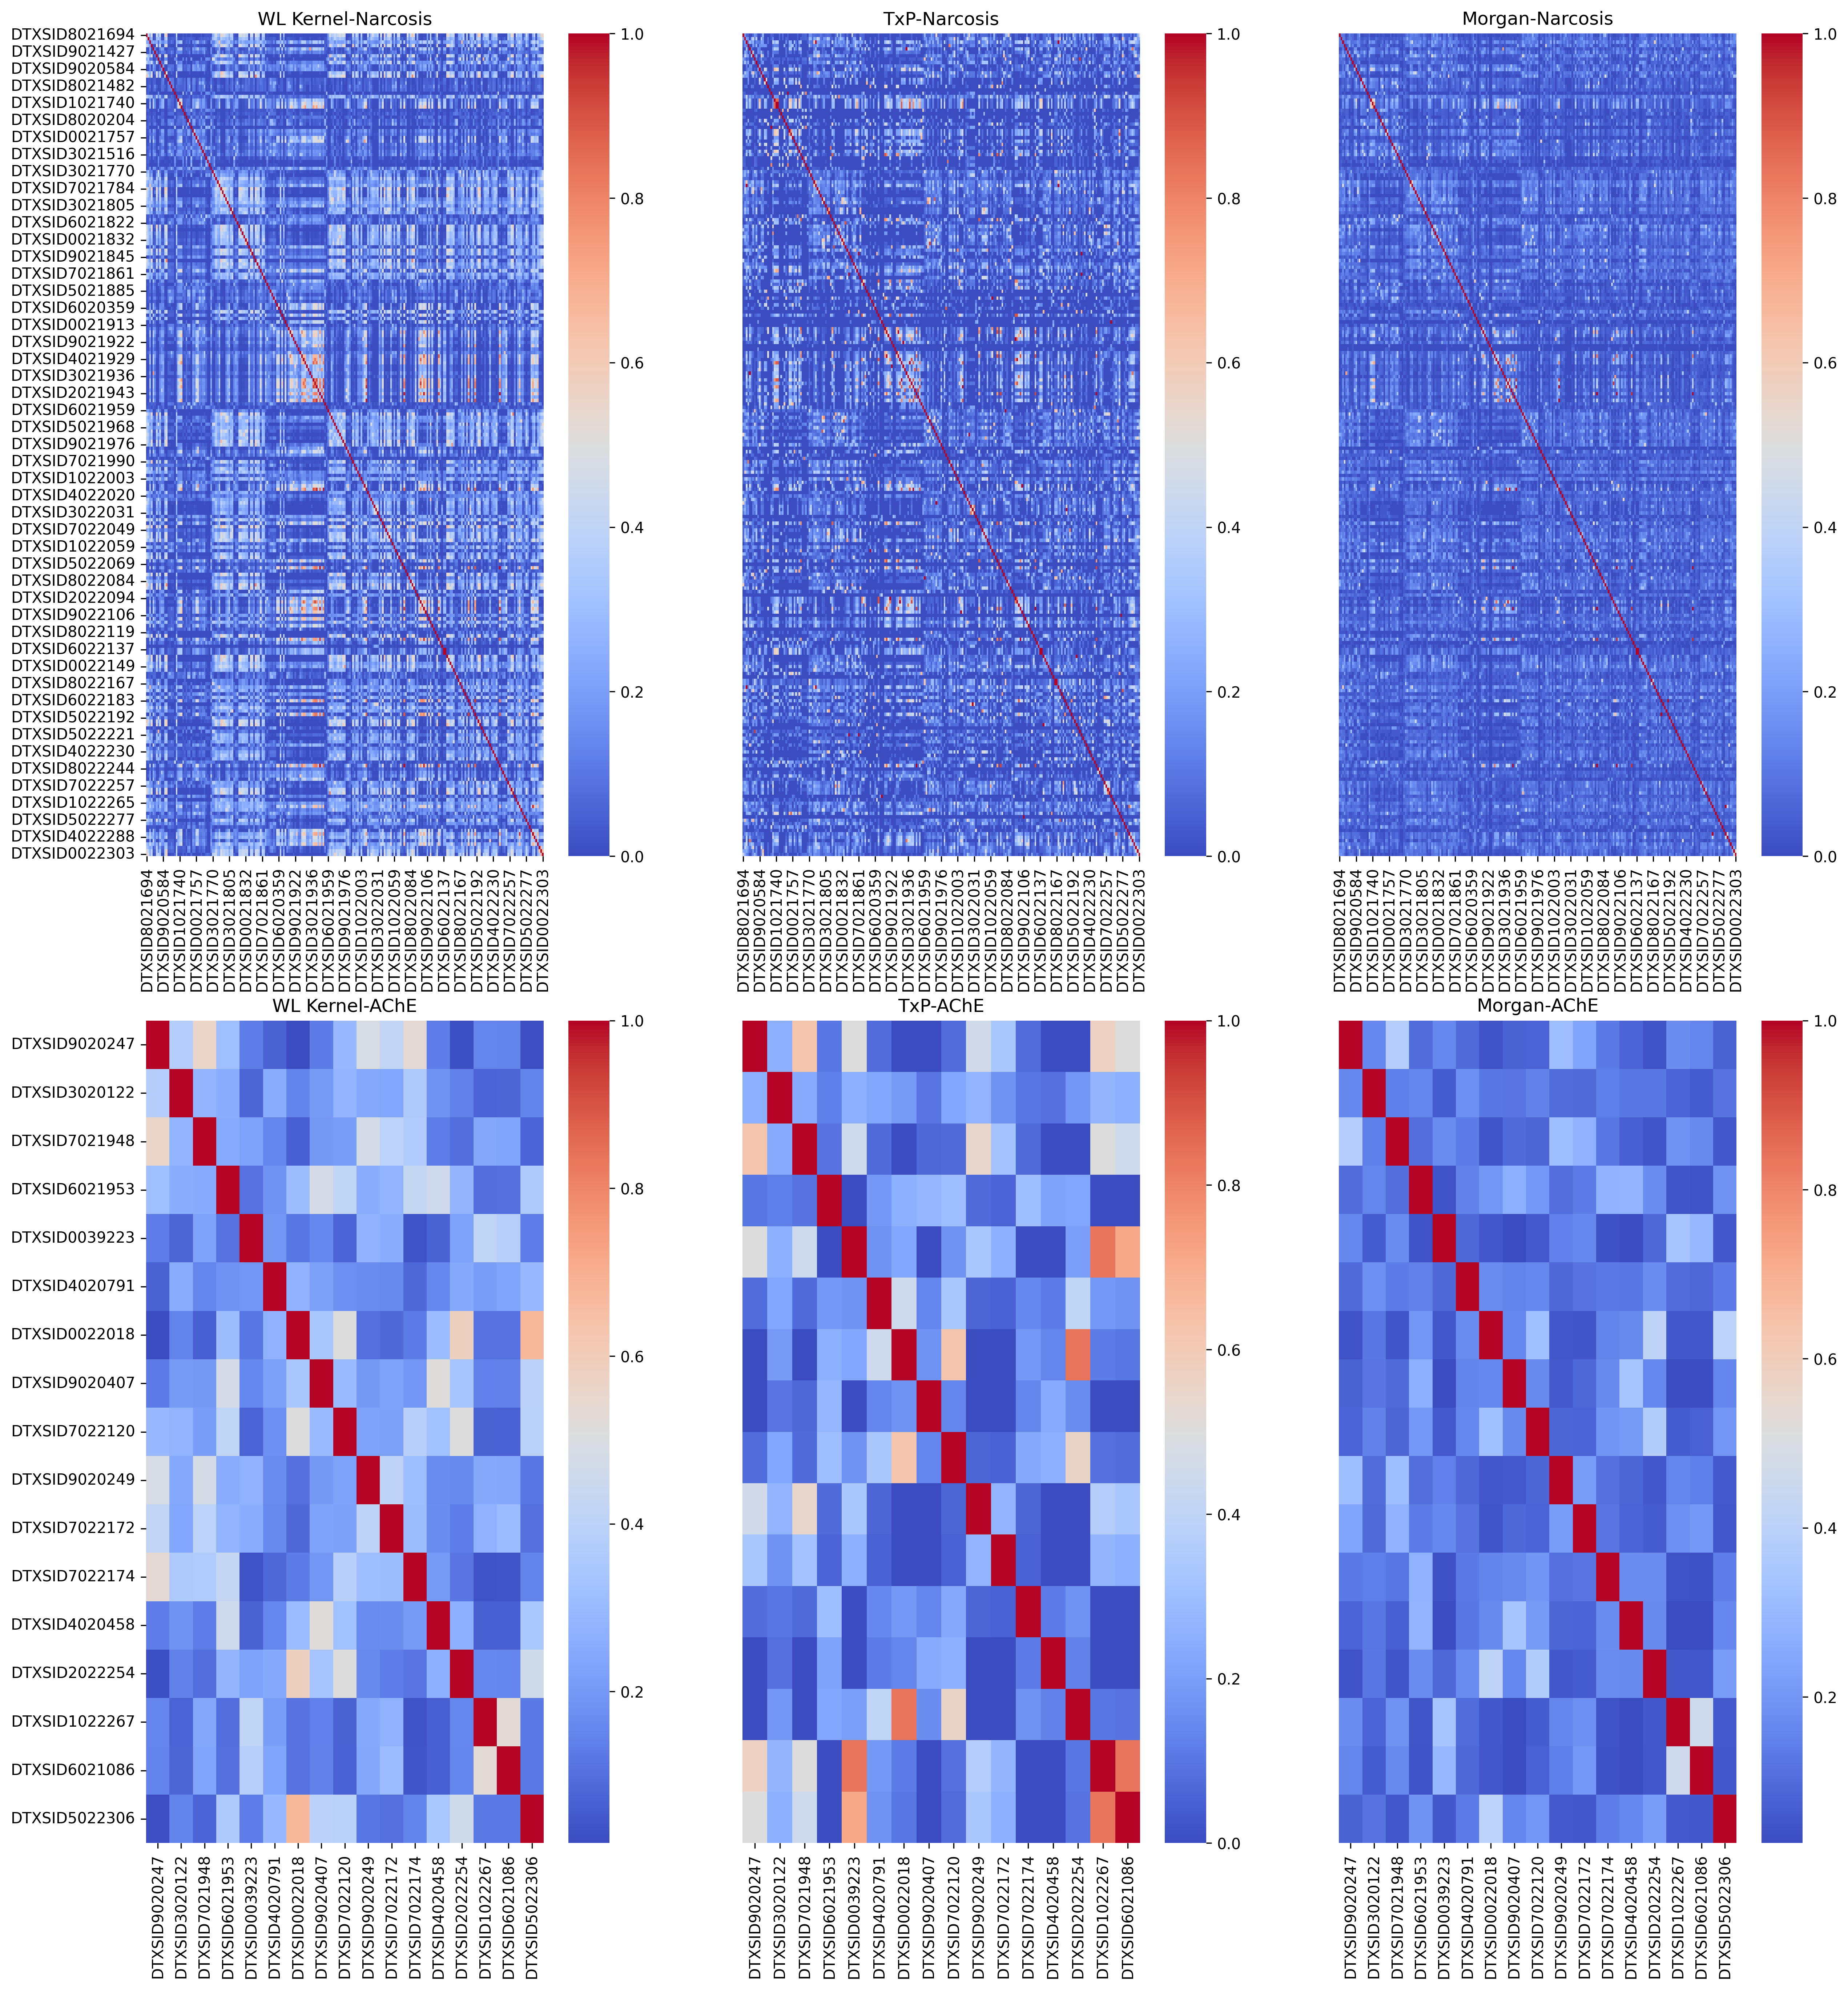
\includegraphics{fhm_sim.png}

}

\caption{\label{fig-fhm}Pairwise similarity matrices across the 3
approaches for the FHM dataset. The pockets of oranges throughout the
matrix highlight those pairs of chemicals that are most similar to each
other. The frequency of the orange squares is more pronounced in the WL
heatmap for substances acting as baseline narcotics whereas there are
more examples of similar AChE pairs using ToxPrints}

\end{figure}%

As an example substance, the top 4 analogues for 1-Bromoheptane
(DTXSID7022095) (nominally assigned as a baseline narcotic) were
retrieved on the basis of the WL scores. Pairwise similarities for the
analogues; 1-Bromohexane (DTXSID4021929), 1-Octanamine (DTXSID8021939),
1-octanol (DTXSID7021940), 1-Bromooctane (DTXSID3021938) all exceeded
0.78. However these pairwise similarities differed to a much greater
extent if ToxPrints formed the basis of the representations. 1-Octanol
and 1-octanamine had much lower similarities due to the different
functional groups present relative to target 1-bromoheptane, yet all
substances were presumed to act as baseline narcotics. For this dataset,
ToxPrints appear to be better able to discriminate substances where
specific functional groups were significant in characterising the MOA,
such as the case for the AChE domain whereas the broader more general
baseline narcosis domain benefited from the WL kernel representation to
identify promising candidate analogues.

\begin{longtable}[]{@{}cccc@{}}
\toprule\noalign{}
Name & Role & WL & TxP \\
\midrule\noalign{}
\endhead
\bottomrule\noalign{}
\endlastfoot
1-bromoheptane (DTXSID7022095) & Target & 1.0 & 1.0 \\
1-bromooctane (DTXSID3021938) & Analogue & 0.93 & 0.91 \\
1-bromohexane (DTXSID4021929) & Analogue & 0.86 & 1.0 \\
1-octanol (DTXSID7021940) & Analogue & 0.78 & 0.36 \\
1-octanamine (DTXSID8021939) & Analogue & 0.78 & 0.36 \\
\end{longtable}

\subsubsection{PPRTV}\label{pprtv}

A read-across example, comprising target substance
2-Amino-4,6-dinitrotoluene (2-ADNT) (CASRN 35572-78-2) and its
structural analogues, was identified from one of the published EPA
Provisional Peer-Reviewed Toxicity Values (PPRTV) assessments. A PPRTV
is defined as a toxicity value derived for use in the EPA Superfund
Program. PPRTVs are derived after a review of the relevant scientific
literature using established EPA Agency guidance on human health
toxicity value derivations. The objective is to provide support for the
hazard and dose-response assessment pertaining to chronic and subchronic
exposures of substances of concern, to present the major conclusions
reached in the hazard identification and derivation of the PPRTVs, and
to characterise the overall confidence in these conclusions and toxicity
values. Current assessments can be accessed on the U.S. Environmental
Protection Agency's (EPA's) PPRTV website at https://www.epa.gov/pprtv.
In cases where there is a paucity of data to derive a PPRTV for a
specific substance, an analogue approach is applied which permits the
use of data from related substances to calculate a screening value. The
exact procedure is described in more detail in Wang et al
\citep{wang_application_2012}.

Five structural analogues with relevant oral non cancer toxicity values
were identified for the target substance 2-ADNT (see
Table~\ref{tbl-pprtv}).

Table~\ref{tbl-pprtv} compares the WL scores with the Jaccard
similarities based on Morgan and ToxPrint fingerprints.

\begin{longtable}[]{@{}
  >{\centering\arraybackslash}p{(\columnwidth - 10\tabcolsep) * \real{0.2000}}
  >{\centering\arraybackslash}p{(\columnwidth - 10\tabcolsep) * \real{0.1600}}
  >{\centering\arraybackslash}p{(\columnwidth - 10\tabcolsep) * \real{0.1600}}
  >{\centering\arraybackslash}p{(\columnwidth - 10\tabcolsep) * \real{0.1600}}
  >{\centering\arraybackslash}p{(\columnwidth - 10\tabcolsep) * \real{0.1600}}
  >{\centering\arraybackslash}p{(\columnwidth - 10\tabcolsep) * \real{0.1600}}@{}}
\caption{2-ADNT is denoted as the target substance based on its role
designation. TNT was ultimately selected as the read-across candidate
out of the 5 candidate analogues. WL, TxP and Morgan denote the
similarity scores computed. WL relies on molecular graphs constructed
using only atoms and other atom property information. The pairwise
scores are shown in each case. e.g.~TNT was determined to have a Jaccard
similarity with 2-ADNT of 0.57 with Morgan fingerprints and 0.67 with
ToxPrints whereas the WL score was
0.69.}\label{tbl-pprtv}\tabularnewline
\toprule\noalign{}
\begin{minipage}[b]{\linewidth}\centering
Substance
\end{minipage} & \begin{minipage}[b]{\linewidth}\centering
Role
\end{minipage} & \begin{minipage}[b]{\linewidth}\centering
DTXSID
\end{minipage} & \begin{minipage}[b]{\linewidth}\centering
WL
\end{minipage} & \begin{minipage}[b]{\linewidth}\centering
TxP
\end{minipage} & \begin{minipage}[b]{\linewidth}\centering
Morgan
\end{minipage} \\
\midrule\noalign{}
\endfirsthead
\toprule\noalign{}
\begin{minipage}[b]{\linewidth}\centering
Substance
\end{minipage} & \begin{minipage}[b]{\linewidth}\centering
Role
\end{minipage} & \begin{minipage}[b]{\linewidth}\centering
DTXSID
\end{minipage} & \begin{minipage}[b]{\linewidth}\centering
WL
\end{minipage} & \begin{minipage}[b]{\linewidth}\centering
TxP
\end{minipage} & \begin{minipage}[b]{\linewidth}\centering
Morgan
\end{minipage} \\
\midrule\noalign{}
\endhead
\bottomrule\noalign{}
\endlastfoot
2-ADNT & Target & DTXSID6044068 & 1 & 1 & 1 \\
TNT & Selected & DTXSID7024372 & 0.69 & 0.67 & 0.57 \\
2-Methyl-5-nitroaniline & Candidate & DTXSID4020959 & 0.49 & 1 & 0.4 \\
Isopropalin & Candidate & DTXSID8024157 & 0.39 & 0.33 & 0.21 \\
Pendimethalin & Candidate & DTXSID7024245 & 0.46 & 0.37 & 0.24 \\
Trifluralin & Candidate & DTXSID4021395 & 0.36 & 0.26 & 0.23 \\
\end{longtable}

Based on an expert-driven evaluation of the structural, physicochemical,
available toxicokinetic (TK) data, and toxicity data,
2,4,6-Trinitrotoluene (TNT) was actually selected as the `best analogue'
primarily based on its metabolic similarity, structural similarity, and
shared metabolites. The similarity of toxicological outcomes across all
the source analogues established confidence in the toxicologic
read-across for 2-ADNT. TNT was also determined to be the most
health-protective analogue because its point of departure (POD) and
corresponding reference dose (RfD) value were lower than the other
candidate analogues. WL and Jaccard (based on Morgan fingerprints)
pairwise similarities across the target and all analogues are shown in
Figure~\ref{fig-pprtv}. TNT had both the highest WL score and Jaccard
similarity on the basis of Morgan fingerprints. ToxPrints identified
2-methyl-5-nitroaniline as more similar on account of the number of
repeating functional groups. Overall based on the highest WL score, TNT
would have been prioritised as the most promising candidate analogue.
However, that is not to say that the representation captures the other
considerations that factored into its selection for the read-across of
2-ADNT.

\begin{figure}

\centering{

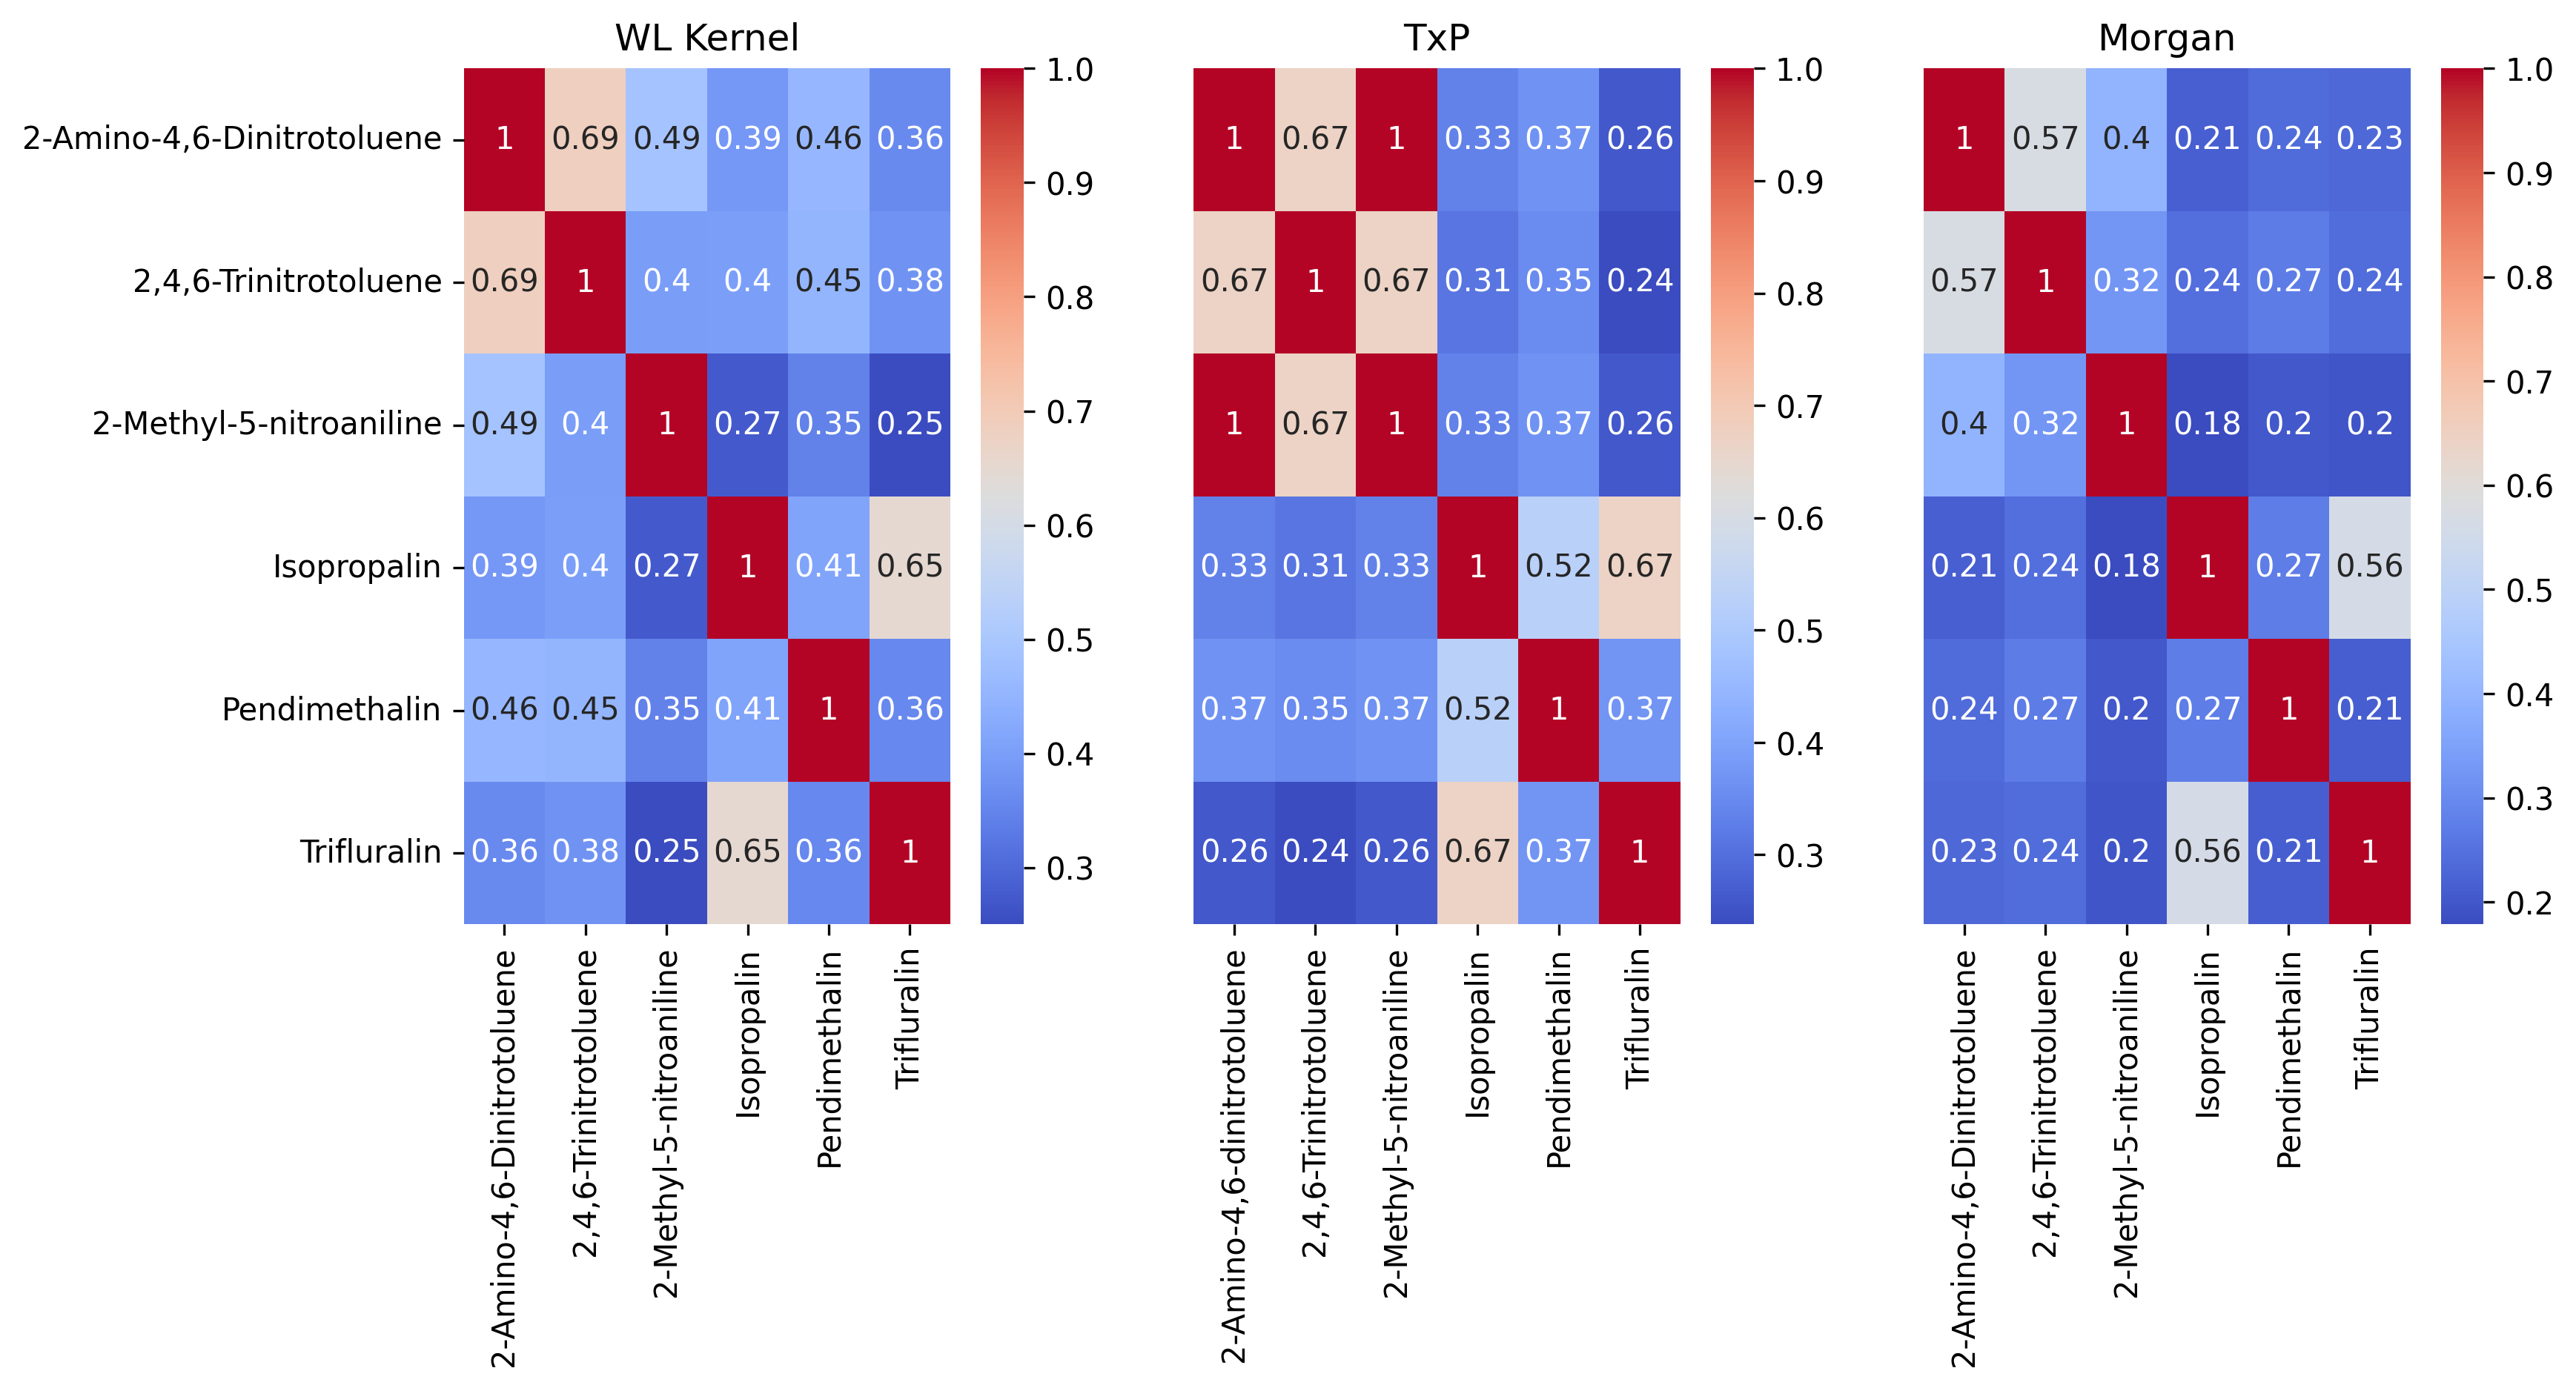
\includegraphics{pprtv_sim.png}

}

\caption{\label{fig-pprtv}Pairwise similarity matrices across the 3
approaches for 2-ADNT and its source analogues.}

\end{figure}%

Across 3 structurally diverse hetereogenous datasets (LLNA, BfR and
FHM), WL was able to differentiate between structurally similar and
dissimilar substances better than Morgan fingerprints and to some extent
ToxPrints. WL iteratively relabels node information thereby capturing
information about the atoms and the topology of the molecular graph. A
refinement to the approach could consider adding bond information as
another attribute in the node labels so that analogues could be refined
further. This could better differentiate between certain functional
groups especially those activated by an unsaturated bond e.g.~alpha,
beta-unsaturated aldehydes vs.~alkyl aldehydes. When datasets were
stratified by MOA or reaction chemistry that was well aligned with
specific functional groups such as those indicative of electrophilic
features, ToxPrints fared better at differentiating between chemicals.
ToxPrints fare poorly when the presence of multiple functional groups is
a factor e.g.~2-ADNT and 2-methyl-5-nitroaniline were considered the
same on account of the nitro group but the dinitro moiety would confer
some different reaction chemistry. Based on the insights derived from
exploring these datasets, WL does show promise in identifying candidate
analogues but only where reactive chemistry is not a determining factor
for the toxicity concerned.

\subsection{Unsupervised graph
embeddings}\label{unsupervised-graph-embeddings}

\subsubsection{Graph2Vec}\label{graph2vec}

Given WL focused on relabelling of nodes alone, Graph2Vec was next
investigated in an attempt to learn graph-level embeddings of the
substances within both the LLNA and FHM datasets. These datasets were
chosen since they were modest in size. t-SNE 2D projections
\citep{van_er_maaten_visualizing_2018} colour coded by the reaction
domains (Figure~\ref{fig-g2vllna}) (or MOA data not shown) showed no
obvious clustering of the substances. Whilst a disappointing result, it
does suggest that neither dataset was sufficiently large enough to
permit a more generalised vocabulary of substructures and patterns to be
generated in order to capture nuanced differences from the substances.
Accordingly to make better use of the Graph2Vec technique, a much larger
dataset of substances would be needed to learn useful embeddings.

\begin{figure}

\centering{

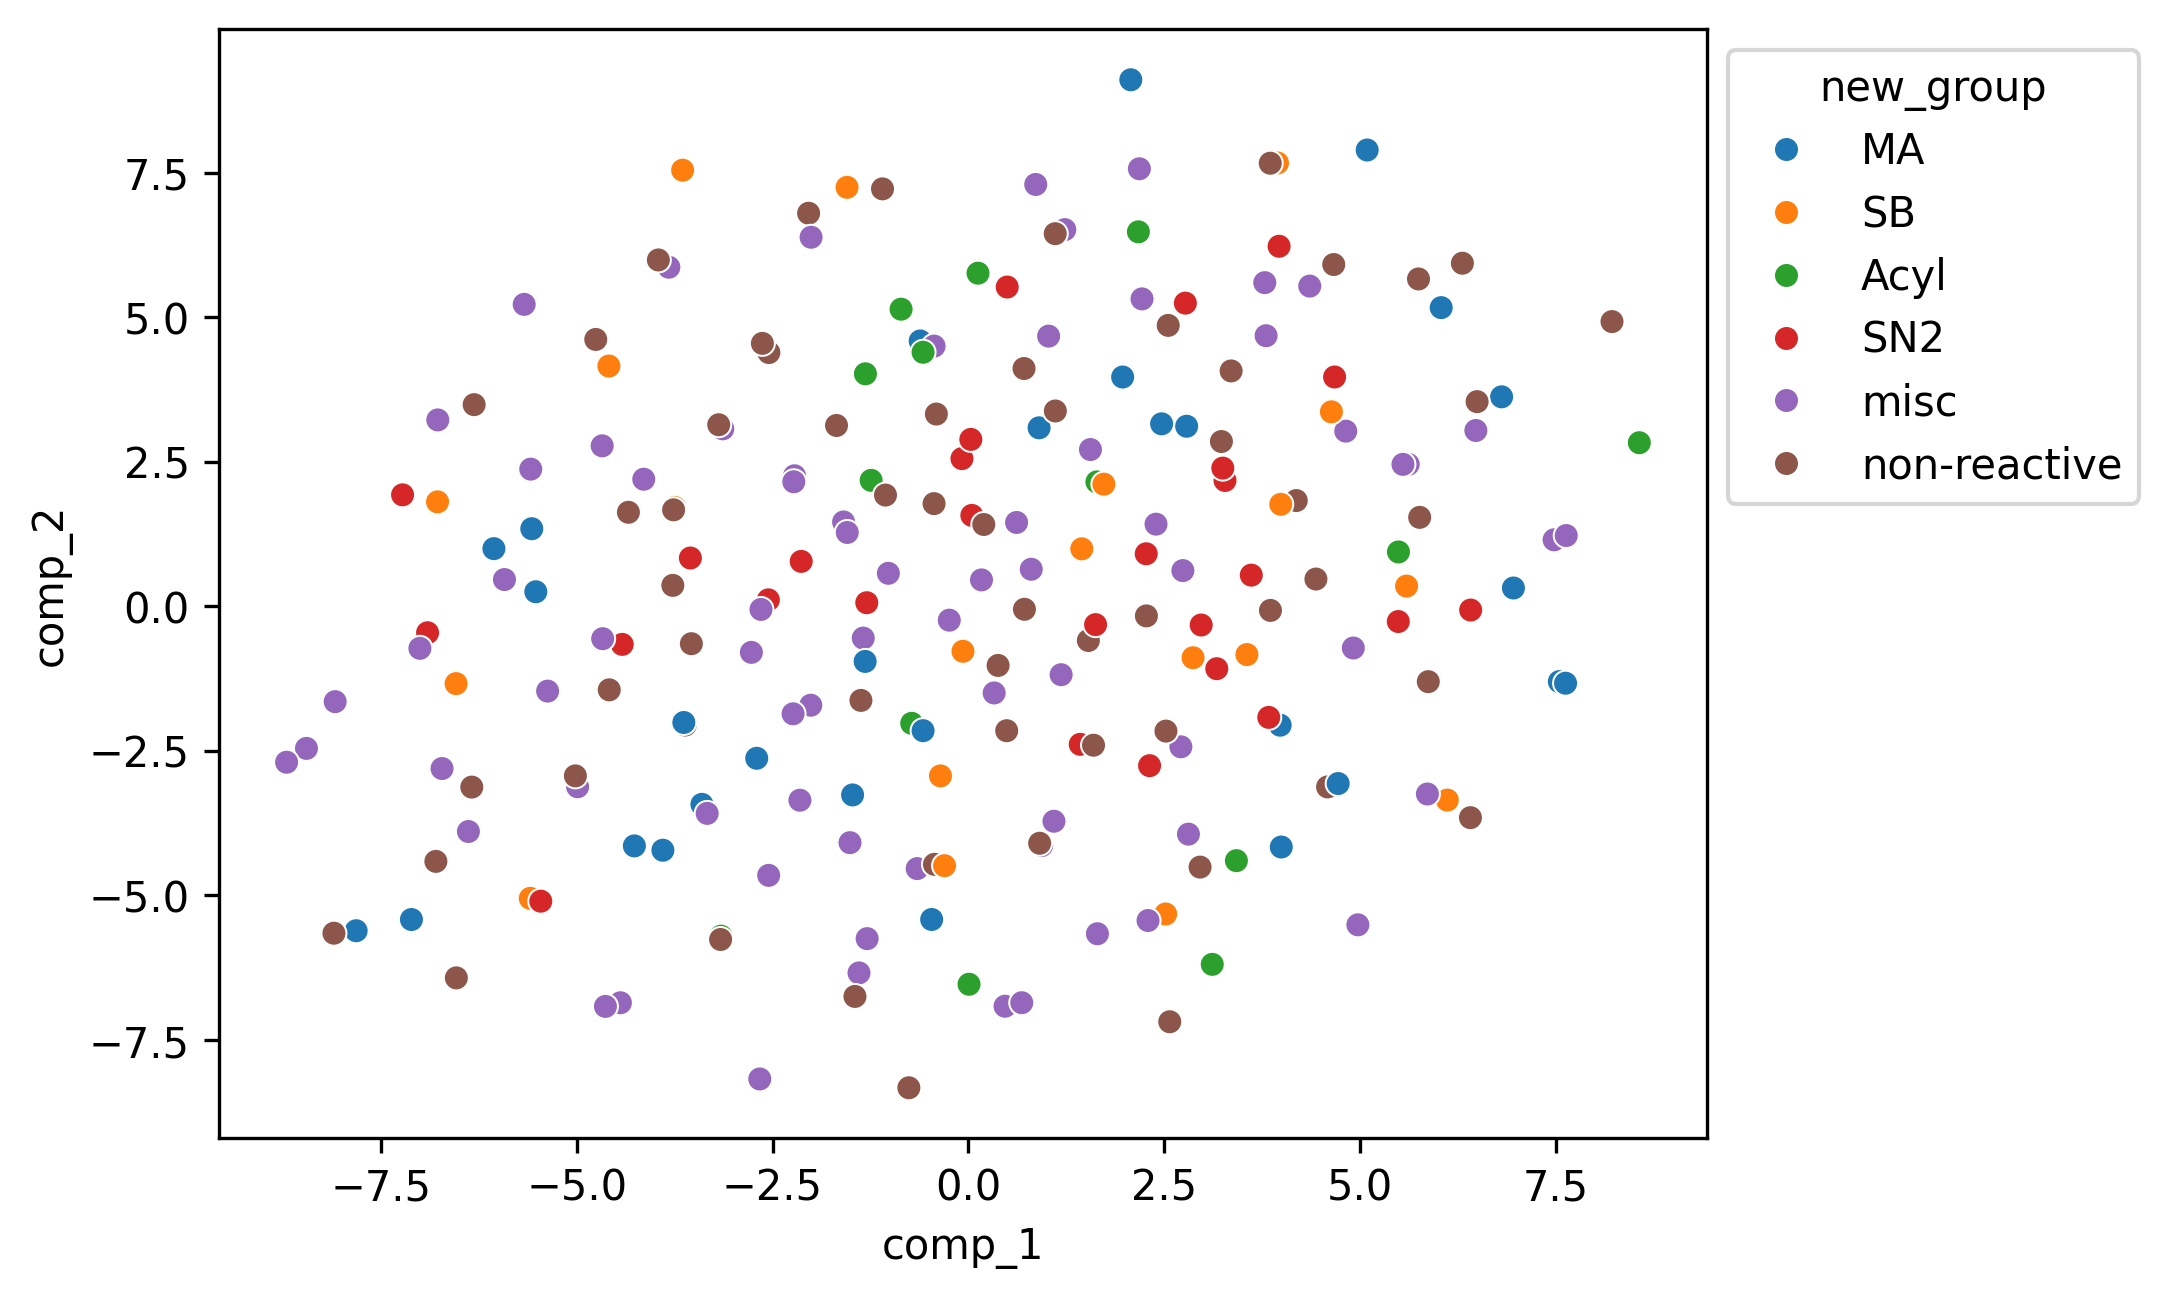
\includegraphics{tsne_llna_graph2vec.png}

}

\caption{\label{fig-g2vllna}TSNE plot of embeddings from Graph2Vec}

\end{figure}%

A case in point was that for 1-Bromoheptane (DTXSID7022095), the top 4
analogues based on the Graph2Vec embeddings and their cosine distance
(range 0.45-0.47) were 2-Methoxyethylamine (DTXSID1021908),
2,3-Dihydrobenzofuran (DTXSID2022040), Methyl tert-butyl ether
(DTXSID3020833) and 2-Chloro-1-methylpyridinium iodide (DTXSID6022260).
Contrasting that were the cosine distances for the source analogues
identified by using a WL kernel as discussed in Section~\ref{sec-fhm}
(see Table~\ref{tbl-fhm-g2v}) which were all quite high (cosine distance
ranging from 0-2) demonstrating that the embeddings did not determine
these source analogues as being particularly similar.

\begin{longtable}[]{@{}cccc@{}}
\caption{WL similarities and cosine distances derived from Graph2Vec
embeddings for WL-identified analogues of 1-bromoheptane as taken from
the FHM dataset.}\label{tbl-fhm-g2v}\tabularnewline
\toprule\noalign{}
Name & Role & WL & Graph2Vec \\
\midrule\noalign{}
\endfirsthead
\toprule\noalign{}
Name & Role & WL & Graph2Vec \\
\midrule\noalign{}
\endhead
\bottomrule\noalign{}
\endlastfoot
1-bromoheptane (DTXSID7022095) & Target & 1.0 & 0.0 \\
1-bromooctane (DTXSID3021938) & Analogue & 0.93 & 0.70 \\
1-bromohexane (DTXSID4021929) & Analogue & 0.86 & 0.81 \\
1-octanol (DTXSID7021940) & Analogue & 0.78 & 0.63 \\
1-octanamine (DTXSID8021939) & Analogue & 0.78 & 0.66 \\
\end{longtable}

\subsubsection{Mol2Vec}\label{mol2vec}

The Mol2Vec model derived from DSSTox structures was then applied to
both the LLNA and FHM datasets from which distance matrices using cosine
as a metric were generated. Pairwise distances were explored for the
entire dataset as well as different reaction domains/MOAs.

Considering the same pairs of substances as in Section~\ref{sec-llna},
pairwise cosine distances were found to be very low suggesting that the
embeddings were able to resolve high similarities between the pairs in
Table~\ref{tbl-llnam2v}.

\begin{longtable}[]{@{}
  >{\centering\arraybackslash}p{(\columnwidth - 8\tabcolsep) * \real{0.1064}}
  >{\centering\arraybackslash}p{(\columnwidth - 8\tabcolsep) * \real{0.3404}}
  >{\centering\arraybackslash}p{(\columnwidth - 8\tabcolsep) * \real{0.3404}}
  >{\centering\arraybackslash}p{(\columnwidth - 8\tabcolsep) * \real{0.1064}}
  >{\centering\arraybackslash}p{(\columnwidth - 8\tabcolsep) * \real{0.1064}}@{}}
\caption{Pairwise similarities based on ToxPrint fingerprints and cosine
distances from Mol2Vec embeddings for selected substances from the LLNA
dataset}\label{tbl-llnam2v}\tabularnewline
\toprule\noalign{}
\begin{minipage}[b]{\linewidth}\centering
Reaction domain
\end{minipage} & \begin{minipage}[b]{\linewidth}\centering
\end{minipage} & \begin{minipage}[b]{\linewidth}\centering
\end{minipage} & \begin{minipage}[b]{\linewidth}\centering
Mol2Vec
\end{minipage} & \begin{minipage}[b]{\linewidth}\centering
ToxPrint
\end{minipage} \\
\midrule\noalign{}
\endfirsthead
\toprule\noalign{}
\begin{minipage}[b]{\linewidth}\centering
Reaction domain
\end{minipage} & \begin{minipage}[b]{\linewidth}\centering
\end{minipage} & \begin{minipage}[b]{\linewidth}\centering
\end{minipage} & \begin{minipage}[b]{\linewidth}\centering
Mol2Vec
\end{minipage} & \begin{minipage}[b]{\linewidth}\centering
ToxPrint
\end{minipage} \\
\midrule\noalign{}
\endhead
\bottomrule\noalign{}
\endlastfoot
MA & Ethyl acrylate (DTXSID4020583) & Butyl acrylate (DTXSID6024676) &
0.0096 & 0.66 \\
MA & trans-2-decenal (DTXSID5047035) & trans-2-hexenal (DTXSID1041425) &
0.015 & 0.86 \\
Acyl & Phthalic anhydride (DTXSID2021159) & Trimellitic anhydride
(DTXSID7026235) & 0.0067 & 0.7 \\
\end{longtable}

However closer inspection of the cosine distance matrix revealed very
little variation across the entire LLNA dataset. In fact,
\textasciitilde94\% of the pairwise distances were in the range of 0-0.1
whereas the most dissimilar pairs had a cosine distance of up to 0.5.
Searching for the top 5 source analogues for 1-Bromobutane
(DTXSID6021903) identified very unrelated substances at least on their
reaction domain. 1-Bromobutane would react by a SN2 mechanism with
respect to skin sensitisation, whereas the source analogues identified
were either non-reactive or Schiff base formers (DTXSID1021740,
DTXSID6021583, DTXSID6020515 and DTXSID0021206).

For the analogues identified based on WL for 1-bromoheptane, all the
source analogues had a cosine distance of 0.004476-0.005743 but overall
the cosine distance matrix for the FHM dataset had 93\% of its pairwise
distance in the range of 0-0.1 revealing it was unable to discriminate
dissimilar substances effectively.

Accordingly, a much larger corpus to learn the embeddings, in the order
of 10s of million structures as used in the original work vs 1/2 million
diverse structures from DSSTox would be needed to produce meaningful
embeddings that could be then used to extract any useful insights for
the 2 datasets herein. Of note, the original Mol2Vec package had been
archived and it was not possible to recreate the same corpus used in
that study to explore whether any useful embeddings might have been
derived for the 2 datasets here.

Unsupervised whole graph embeddings using Graph2Vec or Mol2Vec appear to
offer the potential to better encode whole molecule information beyond
the more limited capabilities that WL can offer in terms of capturing
local neighbourhoods and atom information. However, for the 2 datasets
explored, the embeddings learned from a `large' dataset of 0.5 million
DSSTox substances proved woefully insufficient to be able to resolve
differences in structure that could be useful from a read-across
perspective.

\subsection{Graph Embedding}\label{sec-graph2vec}

As a final attempt to explore the utility of the graph embedding
approach, a larger dataset of genotoxicity outcomes was used. The
genotoxicity dataset was an updated version of that compiled in Pradeep
et al \citep{pradeep_evaluation_2021} drawn from the EPA Toxicity Values
database (ToxValDB). The same methodology as described in Pradeep et al
\citep{pradeep_evaluation_2021} was used to create a dataset with a
summary genotoxicity outcome for each chemical. Genotoxicity studies,
including \emph{in vitro} and \emph{in vivo} chromosomal aberration,
Ames, micronucleus, mouse lymphoma studies were initially retrieved from
ToxValDB. To create a single outcome per chemical, the dataset was first
grouped by substance identifier and summarized as follows: if a
substance was associated with a positive Ames result, a positive
genotoxicity outcome was returned, if a substance was not associated
with a positive Ames but did have a reported positive chromosomal or
micronucleus outcome, it was tagged as a clastogen. If only inconclusive
studies were associated with a substance, an inconclusive tag was
assigned, finally if only negative outcomes were associated with the
substance, a non-genotoxicity outcome was returned. For the dataset
compiled with structural information, there were 5403 chemicals with
QSAR-READY SMILES and a genotoxicity outcome.

Vectorised embeddings for each substance were derived using Graph2Vec
embedding models. The embeddings were projected in 2D using a
t-distributed stochastic neighborhood embedding (t-SNE)
\citep{van_er_maaten_visualizing_2018}, which was color coded by
genotoxicity outcome. Figure~\ref{fig-g2vgene} shows the 2D projection
though again there was little if any discrimination between positive and
negative outcomes for genotoxicity.

\begin{figure}

\centering{

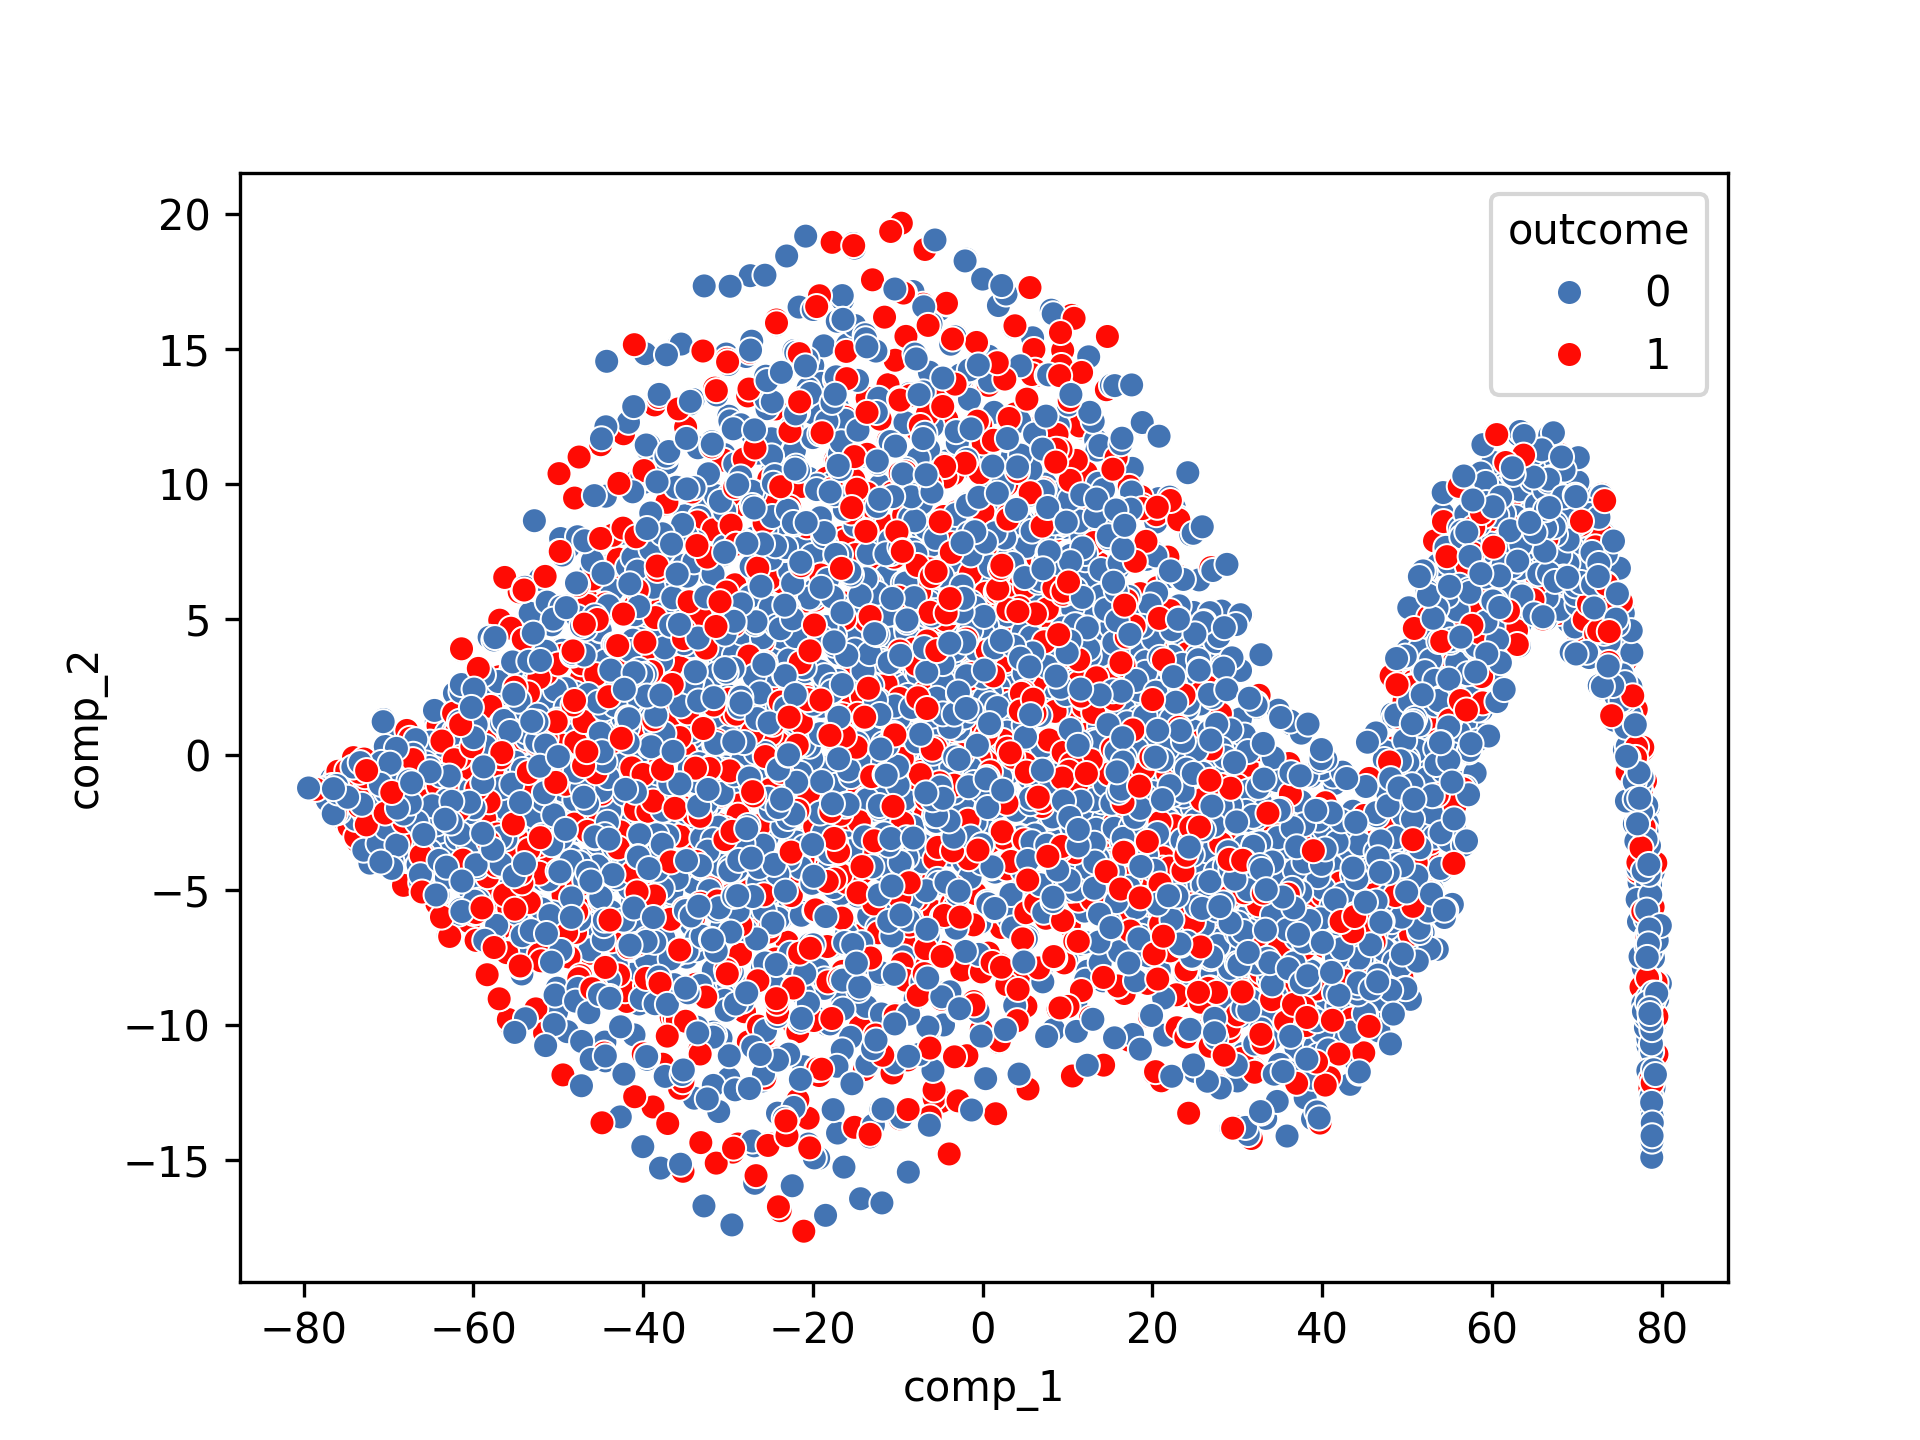
\includegraphics{Graph2Vec_171224.png}

}

\caption{\label{fig-g2vgene}Graph2Vec embeddings projected in 2D TSNE}

\end{figure}%

The embeddings were also used as inputs in 2 classifiers; a k-NN
classifier and logistic regression to assess their informative content.
As a baseline comparator, Morgan chemical fingerprints were used as
feature inputs into the same two classifiers.

\begin{longtable}[]{@{}ccc@{}}
\caption{5-fold cross validated k-nn and logistic regression
genotoxicity classification results using Morgan fingerprints and the
Graph2Vec embeddings method .}\label{tbl-graph2vec}\tabularnewline
\toprule\noalign{}
Embedding Method & K-NN & Logistic Regression \\
\midrule\noalign{}
\endfirsthead
\toprule\noalign{}
Embedding Method & K-NN & Logistic Regression \\
\midrule\noalign{}
\endhead
\bottomrule\noalign{}
\endlastfoot
Morgan FPs & 0.67 & 0.73 \\
Graph2Vec & 0.51 & 0.552 \\
\end{longtable}

The quality of the embeddings generated by Graph2Vec failed to capture
relevant chemical features effectively to be able to discriminate
between genotoxic and non-genotoxic outcomes. Morgan chemical
fingerprints outperformed the graph embeddings using both classifiers
(see Table~\ref{tbl-graph2vec}). Graph2Vec struggled to separate the
data, with almost no discrimination between the two outcomes as shown in
Figure~\ref{fig-g2vgene}. Fine tuning parameters such as embedding
length and learning rates could possibly increase performance since the
embeddings were generated using the default parameters of the model.
Default parameters were also used for the classification models, leaving
another area of possible improvement.

\subsection{GCN Embeddings}\label{gcn-embeddings}

The same dataset as described Section~\ref{sec-graph2vec} was used to
demonstrate the applicability of the GCN embedding method.

GCN embeddings were visualised via t-SNE and labelled by outcome as
shown in Figure~\ref{fig-gcn-nn}. The 5-fold cross validation AUC scores
for the K-NN and Logistic regression using the GCN embeddings were found
to be 0.659 and 0.778 respectively, a comparable performance to Morgan
fingerprints using a K-NN approach but a marked improved with the
logistic regression.

\begin{figure}[H]

\centering{

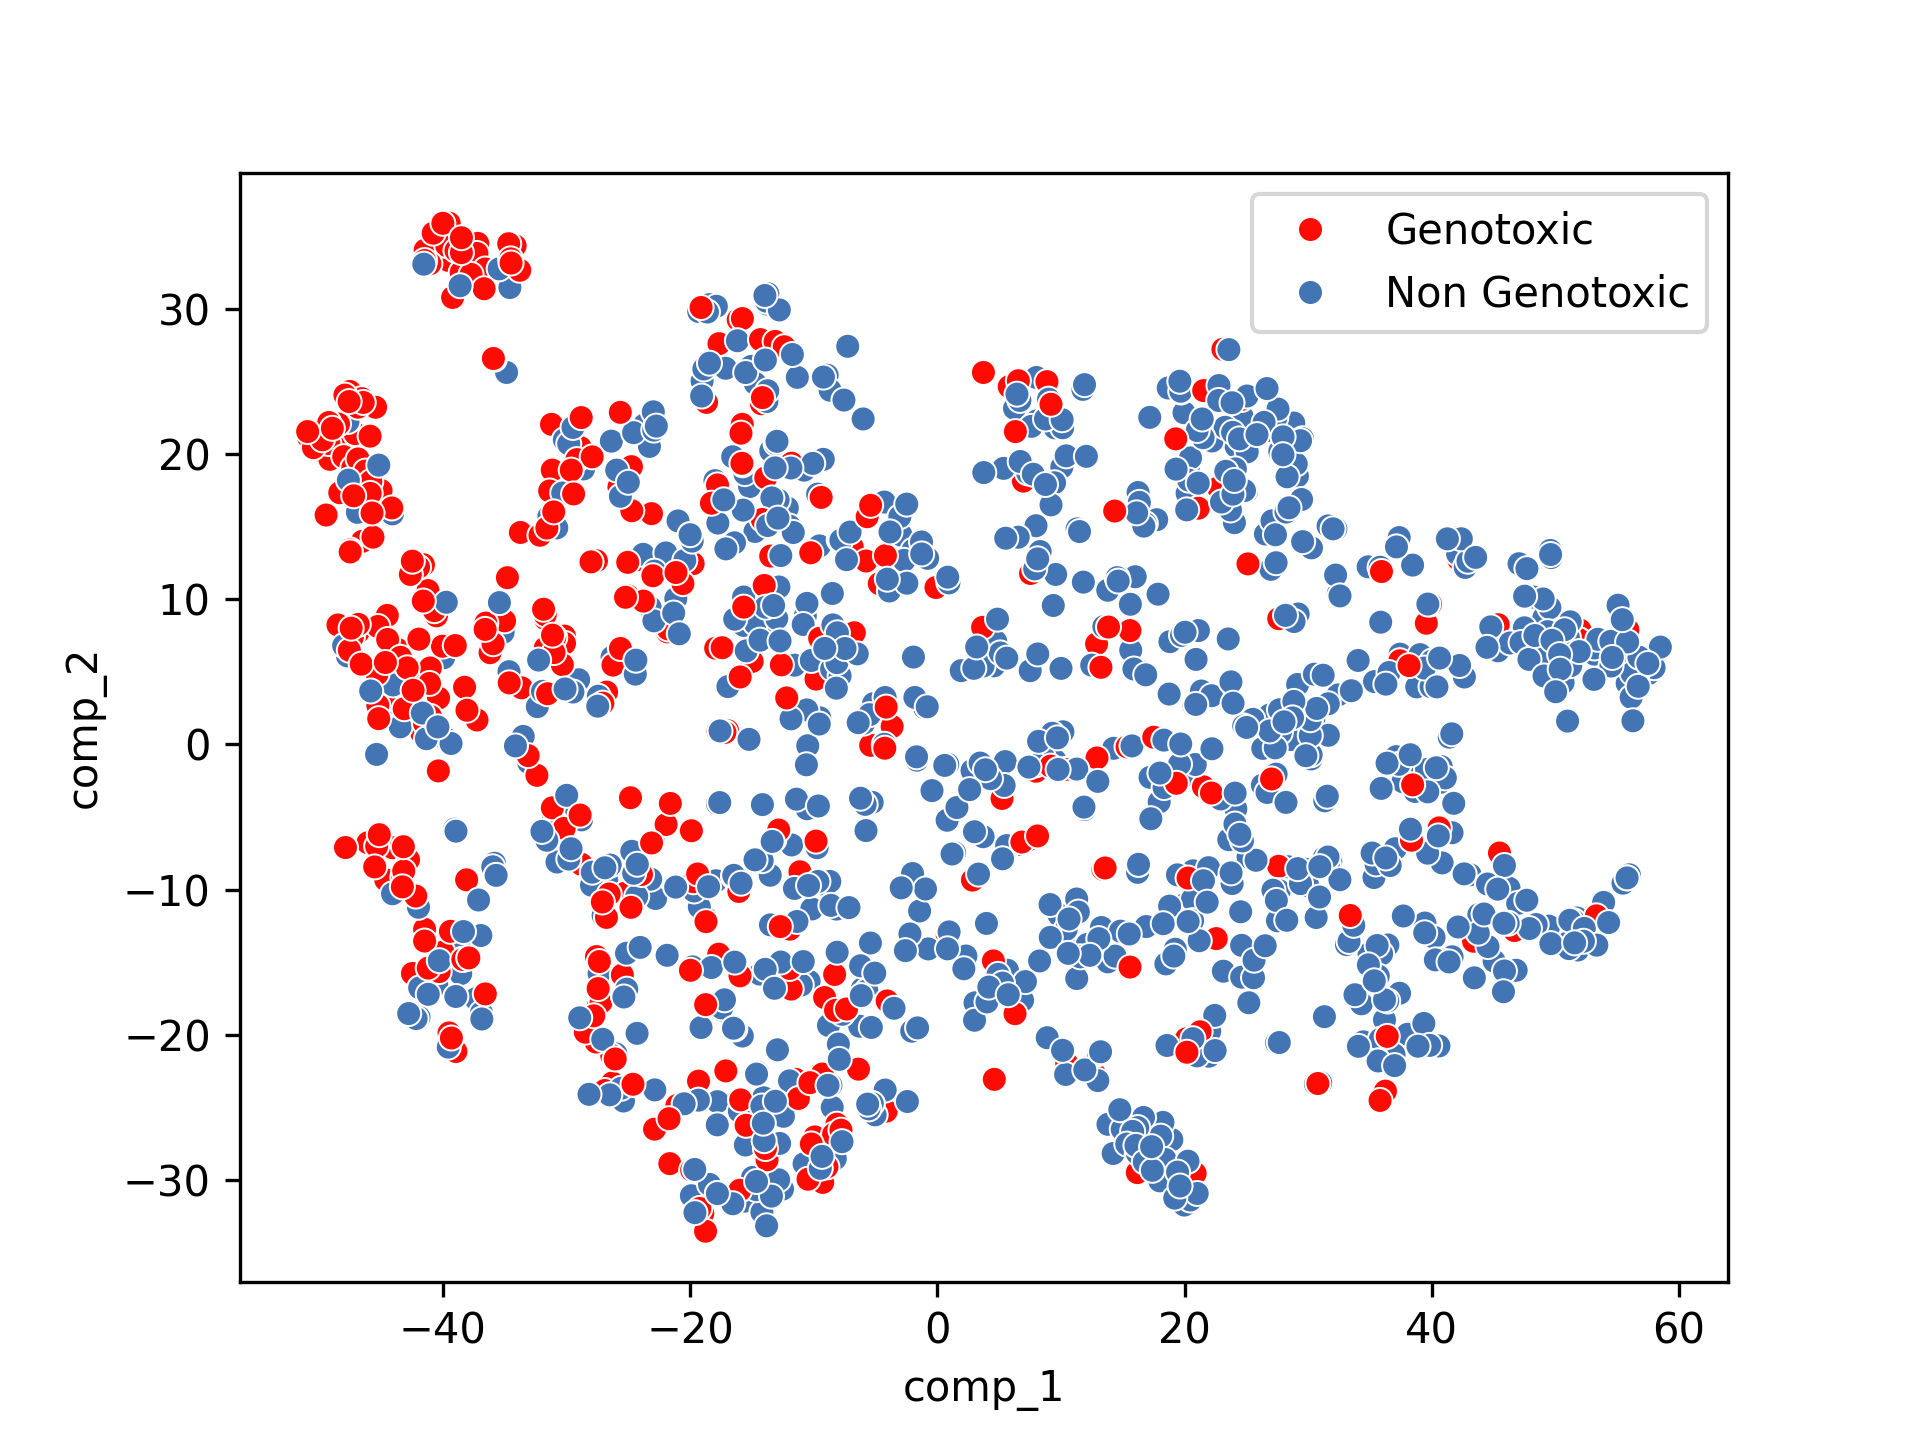
\includegraphics{GCN_embedding_171224.png}

}

\caption{\label{fig-gcn-nn}GCN embeddings of validation graph set
labeled by genotoxicity outcome}

\end{figure}%

As with the previous graph embedding discussed in
Section~\ref{sec-graph2vec}, default parameters were used for both
classification models, likely leaving room for improvement in
performance through hyperparameter tuning. As with all DL models, there
are a large number of options available when constructing a GCN
architecture. Layer types, selection of activation functions, pooling
methods, choice of loss functions and optimizers, as well as the fine
tuning of parameters such as the optimiser's learning rate, the number
of training epochs and number of neurons per layer are all of
significant importance in a network's performance. Further
experimentation with network architecture would likely lead to better
performance, but for the purposes of this illustrative example, the
application of a generically designed network without any fine tuning
was still able to yield reasonable performance.

Taking the embeddings generated for the validation set, and deriving the
cosine metric identified 21.6\% of pairings as falling in the range of
0-0.1 cosine distance, 44.46\% in the 0.1-0.3 distance range, 21\% in
the 0.3-0.5 distance range, 8.4\% in the 0.5-0.7 and 4.3\% in the
0.7-1.0 distance range.

For target substance, 3-Methyl-4-nitroquinoline 1-oxide (DTXSID8074944),
the top 4 closest analogues as shown in Table~\ref{tbl-gcngen} were
identified. Three of analogues were associated with positive genetox
outcomes in concordance with that of the target substance. These source
analogues all contained nitroso moieties known to be associated with
positive genetox outcomes. Whereas the unsupervised whole embedding
approach proved unsuccessful, it was possible to use a much larger
dataset of several thousand substances and use that to extract a learned
embedding that encoded specific features that could discriminate for
genotoxicity. These embeddings proved effective to retrieve similar
analogues that were both structurally and toxicologically related, as
demonstrated for the target DTXSID8074944.

\begin{longtable}[]{@{}ccc@{}}
\caption{Pairwise cosine distances for analogues related to
DTXSID8074944}\label{tbl-gcngen}\tabularnewline
\toprule\noalign{}
& Cosine distance & Genetox outcome \\
\midrule\noalign{}
\endfirsthead
\toprule\noalign{}
& Cosine distance & Genetox outcome \\
\midrule\noalign{}
\endhead
\bottomrule\noalign{}
\endlastfoot
DTXSID8074944 & 0.0 & 1 \\
DTXSID9067980 & 0.05 & 0 \\
DTXSID8020751 & 0.06 & 1 \\
DTXSID8020593 & 0.08 & 1 \\
DTXSID70875601 & 0.08 & 1 \\
\end{longtable}

\section{Conclusion}\label{conclusion}

In this study, a selection of approaches to quantify graph similarity
were investigated using 5 different datasets to better understand their
utility in identifying and evaluating analogues within a read-across
approach compared with 2 conventional chemical fingerprint descriptors.
A WL graph kernel approach was found to be useful in characterising
potential analogues relative to 2-ADNT, identifying TNT as the most
similar analogue. TNT was selected as the source analogue for use in the
read-across assessment. The WL scores were found to be sensitive to the
way in which the graphs were initially constructed such that if atom and
bond characteristics were not sufficiently captured, local differences
in structural representations could be underrepresented relative to the
whole molecular effects and thereby overinflating the resulting scores.
Careful attention is needed to capture node and edge information before
their use. The Jaccard scores using Morgan fingerprints were lower no
doubt highlighting that small changes in substituents and their
positions are not well discriminated across the analogues relative to
the target substance. Topological and label information played a
significant role in ascertaining the WL similarities.

In contrast embedding approaches building on the Mol2Vec approach were
found to be extremely poor at capturing relevant molecular information
to discriminate between substances of different reaction domains or
MOAs. Graph2Vec approaches were also found to be ineffective in
discriminating between substances that were genotoxic or not. Morgan
fingerprints were found to be superior in predicting the genotoxicity
outcomes.

A Deep learning GCN model fared much better, with a marked improvement
in performance compared with Morgan fingerprints for classifying for
genotoxicity outcomes. Whereas the embedding approaches applied were
unsupervised in nature, the GCN required labelled training data to
create informed embeddings to facilitate genotoxicity classification.
This performance increase observed also came at a cost of resources,
complexity and required a much larger dataset for training purposes. The
GCN approach can be computationally expensive, depending on model
parameters, scale of datasets, size of graphs and graph features, and
more.

Overall these datasets helped to illustrate the potential that graph
similarity approaches can play in the identification of suitable
analogues for read-across. WL kernels were most useful for analogue
identification where the endpoint is not mediated by reaction chemistry.
Graph2Vec embeddings were shown to be ineffective in any of the example
datasets despite the potential that whole graph embeddings might have to
capturing structural information. For larger datasets with toxicity
outcomes, GCN approaches produced embeddings informed by genotoxicity
which showed better performance over Morgan type fingerprints and in
identifying relevant analogues. Depending on use case and availability
of training data, graph similarity could play a larger role in analogue
identification and evaluation for read-across. Future work will consider
the role that graph based approaches could play in encoding other types
of information beyond structure such as metabolism information for
read-across purposes.

\section*{Disclaimer}\label{disclaimer}
\addcontentsline{toc}{section}{Disclaimer}

This manuscript reflects the opinions of the authors and are not
reflective or the opinions or policies of the US EPA.

\section*{References}\label{references}
\addcontentsline{toc}{section}{References}

\renewcommand{\bibsection}{}
\bibliography{bibliography.bib}

\newpage{}

\newpage
\appendix
\renewcommand{\thefigure}{A\arabic{figure}}
\renewcommand{\thetable}{A\arabic{table}}
\setcounter{figure}{0}
\setcounter{table}{0}

\section{Supplementary information}\label{supplementary-information}

For context, a few of the pertinent terms/definitions associated with
graphs are described. A graph \[ G(V, E) \] is a visual representation
of a collection of nodes (also called vertices depending on domain) and
edges that connect these nodes providing a structure to represent
entities and their relationships. There are three main types of edges
that are typically found in a graph: undirected edges, directed edges
and weighted edges.

Figure~\ref{fig-gg} provides an example of an undirected graph with 5
nodes and 5 edges and the corresponding directed graph.

\begin{figure}

\begin{minipage}{\linewidth}

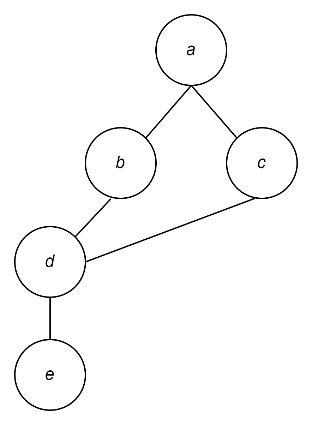
\includegraphics[width=0.3\textwidth,height=\textheight]{fig-gp.png}

\end{minipage}%

\caption{\label{fig-gg}Undirected and directed graph with 5 nodes and 5
edges.}

\end{figure}%

Undirected edges are those which identify a connection between nodes but
without a given ``flow''. Directed edges are those where is a clear
direction between nodes e.g.~within a metabolic graph where a parent
chemical transforms into a metabolite. Weighted edges can occur in both
directed or undirected edges to depict some quantitative value e.g.~the
rate of disappearance of parent chemical to its corresponding
metabolite.

The neighborhood of a node N(v) is the set of all nodes adjacent to v.
In Figure~\ref{fig-gg}, the neighborhood of node d would be expressed as
N(d) = {[}b,c,e{]}. A \emph{walk} comprises a sequence of edges and
nodes, whereas a \emph{path} is a walk with no repeating nodes visited.
In Figure~\ref{fig-path}, the sequence of nodes {[}a,b,d{]} is both a
walk and a path in graph G.

\begin{figure}

\centering{

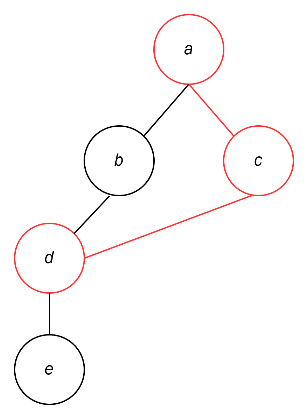
\includegraphics[width=0.3\textwidth,height=\textheight]{fig-path.png}

}

\caption{\label{fig-path}The sequence of nodes {[}a,c,d{]} is both a
walk and a path on G since there are no repeating nodes in the
sequence.}

\end{figure}%

Two graphs are isomorphic if there is a structure that preserves a
one-to-one correspondence between the nodes and edges. In other words,
if the two graphs differ only by the names of the edges and nodes but
are otherwise structurally equivalent, they are said to be isomorphic.





\end{document}
